% % % % % % % % % % % % % % % % % % % % % % % % % % % % % % % % % % % % % % % % % % % %
%                                                                                     %
% Short Sectioned Assignment LaTeX Template Version 1.0 (5/5/12)                      %
% This template has been downloaded from: http://www.LaTeXTemplates.com               %
%                                                                                     %
% Original author:  Frits Wenneker (http://www.howtotex.com)                          %
%                                                                                     %
% Modified by: Fco Javier Sueza Rodríguez (fcosueza@disroot.org)                      %
%                                                                                     %
% Changes:                                                                            %
%	    - Custom Chapters, Sections and Subsections (titlesec package)                %
%           - Document type scrbook (oneside)                                         %
%           - Use babel-lang-spanish package and marvosym                             %
%           - Use hyperref, enumitem, tcolorbox and glossaries packages               %
%           - Use Time New Roman (mathptmx), Helvetic and Courier fonts               %
%                                                                                     %
% License: CC BY-NC-SA 3.0 (http://creativecommons.org/licenses/by-nc-sa/3.0/)        %
%                                                                                     %
% % % % % % % % % % % % % % % % % % % % % % % % % % % % % % % % % % % % % % % % % % % %

%-----------------------------------------------%
%	              Packages                  %
%-----------------------------------------------%

\documentclass[paper=a4, fontsize=11pt, oneside]{scrbook}

% ---- Text Input/Output ----- %

\usepackage[T1]{fontenc}
\usepackage[utf8]{inputenc}
\usepackage{mathptmx}
\usepackage[scaled=.92]{helvet}
\usepackage{courier}
\usepackage[indent=12pt]{parskip}

\usepackage{geometry}
\geometry{verbose,tmargin=3cm,bmargin=3cm,lmargin=2.6cm,rmargin=2.6cm}

% ---- Language ----- %

\usepackage[spanish]{babel}
\usepackage{marvosym}

% ---- Another packages ---- %

\usepackage{amsmath,amsfonts,amsthm}
\usepackage{graphics,graphicx}
\usepackage{titlesec}
\usepackage{fancyhdr}
\usepackage{tcolorbox}
\usepackage{hyperref}
\usepackage{enumitem}
\usepackage[automake]{glossaries}

%--------------------------------------------------------------------%
%                      Customizing Document                          %
%--------------------------------------------------------------------%


% ----------- Custom Chapters, Sections and Subsections -------------- %

\titleformat{\chapter}[display]
			{\bfseries\Huge}
			{Tema \ \thechapter} {0.5ex}
			{\vspace{1ex}\centering}

\titleformat{\section}[hang]
			{\bfseries\Large}
			{\thesection}{0.5em}{}

\titleformat{\subsection}[hang]
			{\bfseries\large}
			{\thesubsection}{0.5em}{}

\titleformat{\subsubsection}[hang]
			{\bfseries\large}
			{\thesubsubsection}{0.5em}{}

\hypersetup{
    colorlinks=true,
    linkcolor=black,
    urlcolor=magenta
}

% ------------------- Custom heaaders and footers ------------------- %

\pagestyle{fancyplain}

\fancyhead[]{}
\fancyfoot[L]{}
\fancyfoot[C]{}
\fancyfoot[R]{\thepage}

\renewcommand{\headrulewidth}{0pt} % Remove header underlines
\renewcommand{\footrulewidth}{0pt} % Remove footer underlines

\setlength{\headheight}{13.6pt} % Customize the height of the header

% --------- Numbering equations, figures and tables ----------------- %

\numberwithin{equation}{section} % Number equations within sections
\numberwithin{figure}{section} % Number figures within sections
\numberwithin{table}{section} % Number tables within sections

% ------------------------ New Commands ----------------------------- %

\newcommand{\horrule}[1]{\rule{\linewidth}{#1}} % Create horizontal rule command


%----------------------------------------------------------------------------------------
%	TÍTULO Y DATOS DEL ALUMNO
%----------------------------------------------------------------------------------------

\title{
\normalfont \normalsize
\textsc{{\bfseries Curso 2022-2023} \\ Ciclo Superior de Desarrollo de Aplicaciones Web \\ IES Aguadulce} \\ [25pt]
\horrule{0.5pt} \\[0.4cm]
\huge Sistemas Informáticos \\
\horrule{0.5pt} \\[0.4cm]
}

\author{Francisco Javier Sueza Rodríguez}
\date{\normalsize\today}

%----------------------------------------------------------------------------------------
%                                     DOCUMENTO
%----------------------------------------------------------------------------------------
\makeglossaries
\loadglsentries{glossary.tex}

\begin{document}

\maketitle

\newpage

\tableofcontents

\listoffigures

%\listoftables

\newpage

\chapter{Hardware de un Sistemas Informático}
En esta primera unidad de la asignatura ``\textbf{Sistemas Informáticos}, vamos a ver los conceptos básicos de sobre los sistemas informáticos, centrándonos principalmente en el apartado del hardware de un sistema informático. Así, veremos cuales son los diferentes componente hardware (o físicos) de un computador, así como la información necesaria para su ensamblaje y puesta en marcha.

También veremos diferentes tipos de clasificaciones de los ordenadores, incluyendo los ordenadores personales, así como otra información útil que podremos encontrar en los diferentes anexos que se incluyen al final de esta unidad.

\section{Sistema Informático}
La \textbf{informática} es la ciencia que se encarga de estudiar todo lo relacionado con los sistemas informáticos, incluyendo los temas relativos a su arquitectura y fabricación, hasta los temas referidos al almacenamiento y organización de la información, sin olvidar la creación y uso de software, o la formación del personal informático. Para ello, se apoya en múltiples disciplinas como las matemáticas, física, electrónica, etc...

Un \textbf{sistema informático} es el conjunto de \textbf{elementos físicos} (hardware) y \textbf{elementos lógicos} (software), interconectados entre sí, destinados a gestionar el \textbf{tratamiento automático de la información}, entendiendo por esto, su almacenamiento, transmisión, organización y/o procesamiento.

Se incluye, como parte fundamental de un sistema informático, al \textbf{conjunto de personas} que lo \textbf{utiliza}, ya sean usuario, administradores, programadores, etc... El elemento humano es un \textbf{componente imprescindible}, ya que los sistemas informáticos son creados, desarrollados y utilizados por humanos para su propio provecho.

En sistema informáticos siempre debemos distinguir entre hardware y software:

\begin{itemize}
    \item \textbf{Hardware}: son todos los elementos físicos que forman parte de un ordenador, es decir, teclado, ratón, placa base, monitor, memoria, disco duro, cables, etc... Es la ``maquinaria'' necesaria utilizada para el tratamiento de la información.
    \item \textbf{Software}: es el elemento lógico e ``intangible'' de un sistema informático. Se compone de un conjunto de programas y datos que permiten manejar el hardware, controlando y coordinando su funcionamiento para que pueda realizar las tareas esperadas. Esta compuesto principalmente de dos elementos:
    \begin{itemize}
        \item \textbf{Programas}: están formados por un conjunto de órdenes o instrucciones que se utilizan para procesador los datos que se introducen como información. Son necesarios para la gestión y el control de los equipos y los trabajos de los usuarios.
        \item \textbf{Datos}: son la información que los programas deben procesar, utilizando para esto diferentes elementos hardware que componen el sistema informático. Son, en definitiva, la razón de ser el sistema informático.
    \end{itemize}
\end{itemize}

Los \textbf{sistemas informáticos} han \textbf{evolucionado}. En un principio todos sus componentes, físicos, lógicos y humanos, estaban localizados en el mismo lugar, pero actualmente están formados por subsistemas que se interconectan a través de la red, que pueden llegar a estar a miles de kilómetros de distancia entre sí, integrando sistemas complejos de procesamiento de la información. Estos subsistemas a si vez pueden estar compuestos por un superodenador, un ordenador personal, redes locales de ordenadores o por una combinación de todos ellos, siendo el sistema informático más simple el formado por un ordenador y un usuario que ejecuta programas en él.

Un \textbf{ordenador} se define como una máquina electrónica, con algunas partes mecánicas, compuesta por al menos, una unidad de proceso, y por equipos periféricos, controlada por programas que deben estar almacenados en su memoria central, destinada al tratamiento automático de la información que le es suministrada. Es una máquina de propósito general ya que puede realizar gran variedad de trabajos y a gran velocidad.

En el \textit{Anexo A.1}, podrás encontrar más información sobre la clasificación de los ordenadores.

\section{Arquitectura Hardware: Componentes Funcionales}
Un computador esta compuesto por una seria de sistemas y subsistemas hardware, que cooperando entre sí, permiten a este llevar a cabo su función, procesando la información que recibe y emitiendo los resultados de este procesado.  En la siguiente figura vemos un esquema de estos subsistemas.

\begin{figure}[ht]
    \centering
    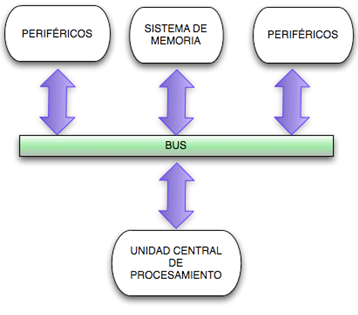
\includegraphics[scale=0.90]{arquitectura-computador.png}
    \caption{Subsistemas de la arquitectura de un computador}
\end{figure}


Como vemos en la imagen, hay tres subsistemas principales, que son los siguientes:

\begin{itemize}
    \item \textbf{Unidad Central de Proceso} (CPU): es el sistemas básico más importante, encargado de coordinar a los demás subsistemas, extraer secuencialmente las instrucciones de la memoria principal para procesarlas y ejecutarlas.
    \item \textbf{Sistemas de Memoria}: su función básica es la de almacenar las instrucciones que se van a procesar posteriormente, los datos y los resultados que sean necesarios.
    \item \textbf{Periféricos}: se dividen en periféricos de entrada y de salida, según la dirección del flujo de información. Ambos sistemas se encargan de la comunicación con el exterior, es decir, con el usuario u otros sistemas.
\end{itemize}

Además de estos tres subsistemas, debemos de hablar de \textbf{bus de sistema}, que es el medio físico encargado de transmitir la información entre los diferentes subsistemas.

En la actualidad, la arquitectura empleada es la fabricación de computadores es la \textbf{arquitectura Von Neumann}. Esta arquitectura de computadoras ésta basada en la descrita en 1945 por el matemático y físico \textbf{John Von Neumann}. En la siguiente imagen podemos ver un esquema de la arquitectura Von Neumann.

\begin{figure}[ht]
    \centering
    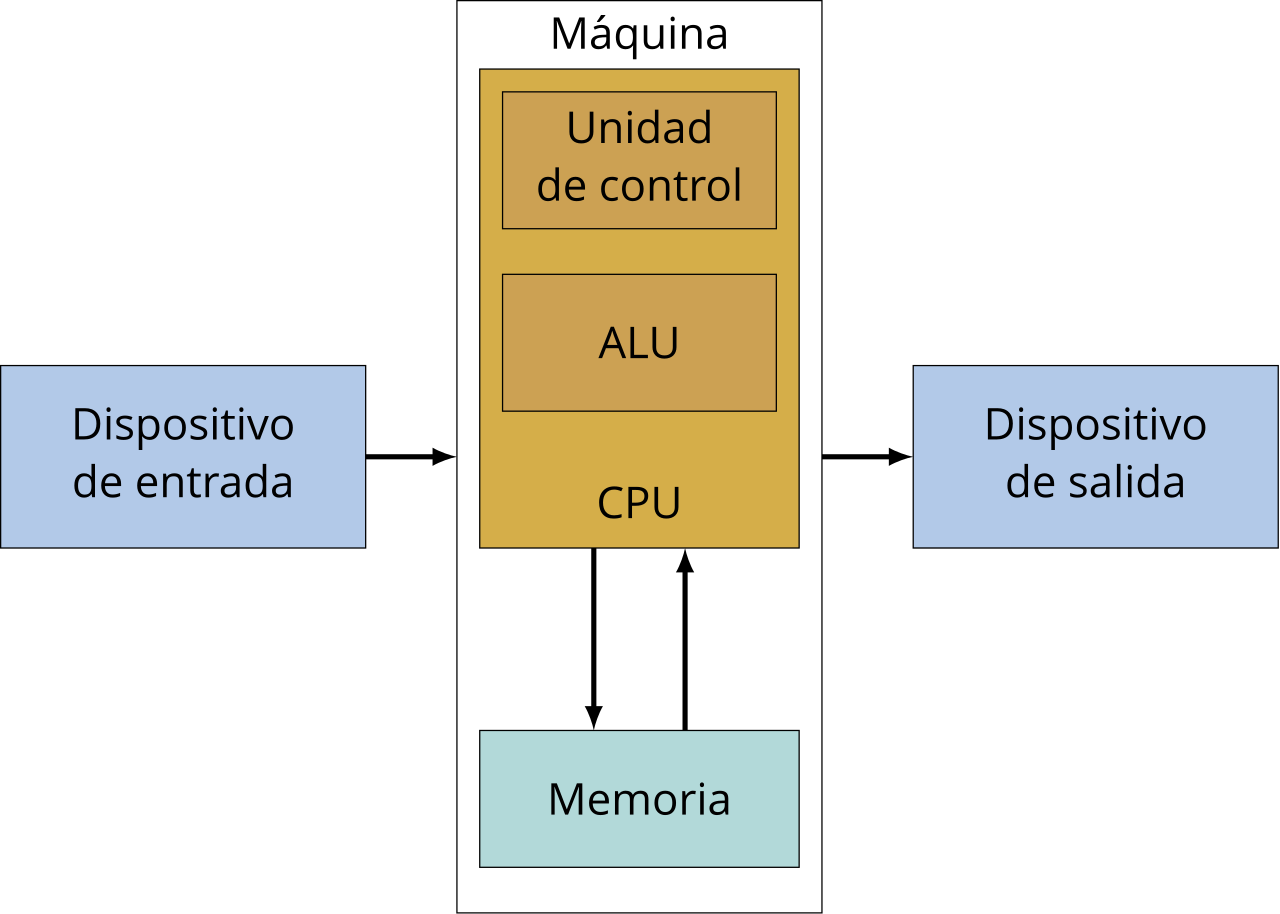
\includegraphics[scale=0.25]{von-neumann.png}
    \caption{Arquitectura Von Neumann}
\end{figure}

Como vemos es igual a la que hemos descrito en este punto. Podemos observar como la \textbf{CPU} contiene dos unidades, la \textbf{unidad de control} y la \textbf{ALU} o \textbf{unidad Aritmético-Lógica}, las cuales veremos con más detalle en la siguiente sección.

Si queremos saber más sobre esta arquitectura, lo cual recomiendo encarecidamente, podemos visitar \href{https://es.wikipedia.org/wiki/Arquitectura_de_Von_Neumann}{la entrada en Wikipedia} de la arquitectura Von Neumann.

\subsection{Componentes Principales (CPU, RAM, E/S, ...)}
La \textbf{Unidad Central de Proceso} es el componente que podría definirse como el ``cerebro'' del computador, ya que es la encargada de controlar, dirigir y coordinar todas las operaciones que realiza el ordenador.

Para que la CPU pueda ejecutar un \textbf{\gls{programa}} es necesario que éste se guarde en su memoria principal, desde donde se van extrayendo en secuencia cada una de sus instrucciones, analizándolas y emitiendo las órdenes necesarias al resto de componentes que deban intervenir para completar su ejecución.

La CPU esta integrada en el Procesador Central o microprocesador y acompañada de una pequeña cantidad de \textbf{\gls{registros}} de memoria necesarios para su funcionamiento.

Dentro del Microprocesador, y como parte integrante de la \textbf{CPU}, existen dos unidades, como ya vimos en el apartado anterior sobre la arquitectura Von Neumann. Esta unidades son:

\begin{itemize}
    \item \textbf{Unidad de Control}: se encarga de ejecutar los programas, controlando su secuencia, interpretando y ejecutando las instrucciones. Se encarga también de controlar al resto de componentes, como periféricos, memoria, etc.., según vayan necesitando las instrucciones.
    \item \textbf{Unidad Aritmético-Lógica} o \textbf{ALU}: se encarga de realiza los cálculos matemáticos y lógicos necesarios para su funcionamiento.
\end{itemize}

La memoria principal, conocida como \textbf{RAM} (Random Access Memory), es la encargada de almacenar los datos e instrucciones de los programas que deben ejecutarse, así como toda la información que el sistema necesita para su funcionamiento. Esta constituida por un \textbf{conjunto de registros} capaces de retener información en su interior mientras el ordenador esta en funcionamiento. Cuando el ordenador se apaga, se pierde su contenido, por lo que esta memoria es de tipo \textbf{\gls{volatil}}.

Los \textbf{sistemas de Entrada y Salida} son circuitos electrónicos que permiten el intercambio de información entre la CPU y los periféricos. Las unidades de entrada y salida se usan para cargar programas y datos en memoria principal desde los periféricos de entrada, y las unidades de salida para mostrar los resultados de las operaciones realizadas a través de periféricos de salida.

Los \textbf{buses del sistema} son el conjunto de circuitos eléctricos que conectan la CPU con el resto de componentes para comunicarse entre sí. Cada bus es un conjunto de cables de un circuito integrado que permite la transmisión de información de forma paralela. Podemos encontrar tres tipos diferentes de buses:

\begin{itemize}
    \item \textbf{Bus de Instrucciones y Datos}: se utilizan para trasladar tanto instrucciones como datos desde la memoria RAM al resto de componentes del computador y viceversa.
    \item \textbf{Bus de Control}: bus que se encarga de trasmitir las instrucciones desde la CPU al resto de unidades y recibe de ellas señales indicando su estado.
    \item \textbf{Bus de Direcciones}: se encarga de transmitir las direcciones de destino de los datos que se envían por el bus de datos.
\end{itemize}

En la siguiente figura, podemos ver un esquema con todos estos componentes.

\begin{figure}[ht]
    \centering
    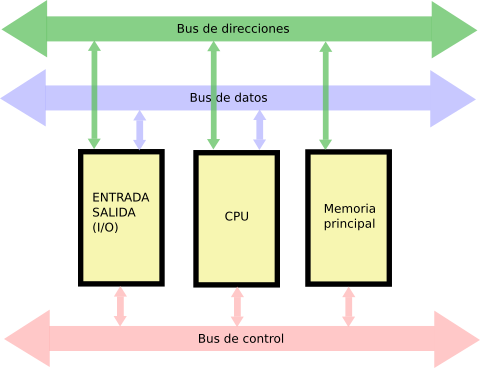
\includegraphics[scale=0.46]{buses-de-sistema.png}
    \caption{Unidades y buses del sistema}
\end{figure}

\subsection{Periféricos y Almacenamiento Externo}
Los \textbf{periféricos} son los dispositivos electrónicos, unidades externas, que se conectan al ordenador a través de los buses de entrada/salida, integrándose en el sistema, que pasa a controlarlos como parte de sí mismo desde el momento en el que se reconoce su conexión.

Existen infinidad de periféricos, diferentes por su diseño y función. Algunos tienen como finalidad facilitar la entrada de información en el ordenador, mientras que otros facilitan su salida, otros cuya finalidad es el almacenamiento permanente de datos o los que permiten la conexión con otras máquinas y el intercambio de información. No todos ellos son imprescindibles, aunque los más normal es contar de teclado, ratón, monitor, impresora altavoces y conexión de red.

Los periféricos se pueden clasificar, según su función, en los siguientes:

\begin{itemize}
    \item \textbf{Unidades de Entrada}: son aquellos periféricos que permiten introducir la información o los datos desde el exterior a la memoria principal, preparando la información para que pueda ser procesada por la máquina. Un ejemplo de estos periféricos son el teclado y el ratón.
    \item \textbf{Unidades de Salida}: son las encargadas de sacar al exterior los datos resultantes de las operaciones realizadas, mostrando la información de forma comprensible para el usuario. Ejemplos de estas unidades son la pantalla o la impresora.
    \item \textbf{Unidades de Entrada/Salida}: esta unidades de usan tanto para entrada como para la salida de información del sistema. Algunas de estas unidades no necesitan hacer procesos de conversión ya que manejan la información en formato binario, mientras que otras necesitan procesos de conversión para trabajar con los usuarios o para comunicarse con otro dispositivo. Algunos ejemplos son las tarjetas de red, discos duros, memorias USB, etc...
\end{itemize}

Algunos periféricos necesitan \textbf{soportes adicionales} para representar la información o almacenarla. En estos casos hay que tener en cuenta que el periférico no almacena la información, sino que es el medio utilizado para obtener o almacenar la información en su soporte. Un ejemplo de esto son los lectores de DVD o Blu-Ray.

\section{Componentes Físicos de un Ordenador Actual}
La arquitectura de un ordenador define la estructura funcional de cada una de sus partes, pero se hace necesario implementar dicha estructura mediante hardware de fabricación y comercialización actual. Dependiendo de  las características tecnológicas de los componentes empleados en su construcción (tamaño, grado de miniaturización, capacidad de procesado, ...), se ensamblarán ordenadores personales más o menos potentes, como portátiles, tablets, smartphones, consolas de juegos, etc... Pero también servidores, mainframes y superordenadores.

Hay que tener en cuenta, que los distintos componentes deben seguir unos estándares de fabricación, especialmente en lo relativo a sus conexiones y \textbf{\gls{interfaces}}, para permitir su completa integración con el sistema y mantener la compatibilidad de funcionamiento entre ellos.

En esta sección vamos a hacer un estudios de los diferentes elementos utilizados para el ensamblaje de un ordenador personal de sobremesa de uso general en base a componentes físicos que se fabrican y comercializan en la actualidad. Analizando en la medida de lo posible sus características de funcionamiento particulares.

\subsection{Cajas de Ordenador}
La \textbf{caja del ordenador}, también conocida como carcasa o chasis, es el ``recipiente'' donde se colocan todos los componentes del ordenador y que sirve para protegerlos. Estas cajas se fabrican en diversos materiales como acero, aluminio, plástico, metacrilato, etc.., o con una combinación de estos. Deben tener la suficiente resistencia para soportar el peso de los componentes en su interior, así como el calor que estos generan y suficiente espacio para albergarlos a todos con una distribución adecuada.

Estás cajas se fabrican siguiendo unos diseños de basados en unos \textbf{factores de forma} estándares, cada uno con sus propias características de tamaño, forma, capacidad, etc. Los principales factores de forma que nos podemos encontrar son los siguientes:

\begin{itemize}
    \item \textbf{Minitorre o Semitorre}: la diferencia entre ellas está en la altura y el número de \textbf{\gls{bahias}} de 5 y cuarto de que dispongan. A mayor número de bahías, más dispositivos podrá contener y más aumenta su altura. Suelen tener entre 2 y 4 bahías respectivamente.
    \item \textbf{Sobremesa}: son similares a las semitorres pero se colocan de forma horizontal, lo que obliga a rotar 90 grados los dispositivos extraíbles de su frontal.
    \item \textbf{Barebone y Slim}: son cajas de pequeño tamaño principalmente diseñadas para ocupar poco espacio. Esto implica que su interior admite pocos dispositivos, o ninguno, pero se compensa aumenta el número de conectores para dispositivos externos.
\end{itemize}

\begin{figure}[ht]
    \centering
    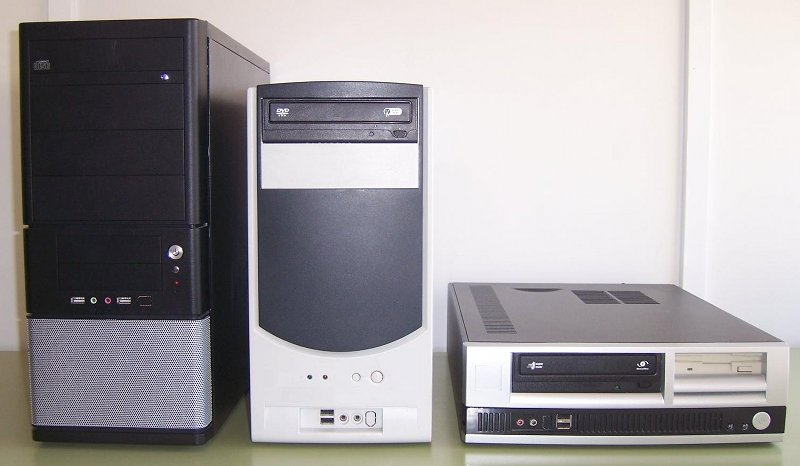
\includegraphics[scale=0.45]{torres-ordenador.jpg}
    \caption{Semitorre, Minitorre y Sobremesa}
\end{figure}

Para ampliar la información sobre los diferentes factores de forma que existen y las características de una caja de ordenador, podemos consultar \href{https://es.wikipedia.org/wiki/Caja_de_computadora}{esta entrada en Wikipedia}.

Independientemente del tamaño o forma que tenga que caja, hay ciertas características que deben tener para cumplir eficientemente su cometido:

\begin{itemize}
    \item En un interior, deben contener \textbf{diferentes compartimentos} dedicados a alojar la fuente de alimentación, los discos duros, las unidades ópticas y por supuesto, la placa base y las tarjetas de expansión que se conecten. En la siguiente figura podemos ver una imagen del interior de una caja (tipo semitorre), donde se pueden observar los diferentes compartimentos que posee.

    \item Deben tener un \textbf{panel frontal}, donde si sitúan los botones de encendido y reinicio, así como los LED que indican si el ordenador esta encendido y si se esta usando el disco duro.

    \item En el \textbf{panel trasero} se deben encontrar los diferentes conectores que vienen desde la placa base y las tarjetas de expansión, así como la toma de corriente.

    \item También deberá tener, distribuidas estratégicamente, \textbf{diferentes rejillas} que ayuden a la disipación del calor que generan los componentes en el interior de la caja.

   \begin{figure}[ht]
        \centering
        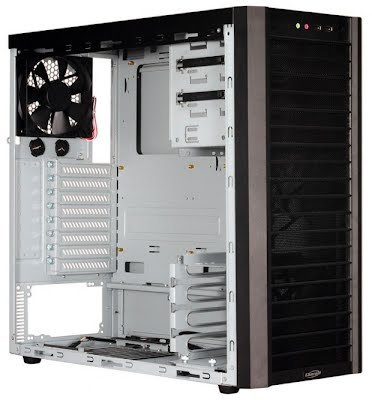
\includegraphics[scale=0.45]{caja-abierta.jpg}
        \caption{Caja de tipo semitorre abierta}
    \end{figure}
\end{itemize}

\subsubsection{Fuente de Alimentación}
La \textbf{fuente de alimentación} es una elemento imprescindible cuya misión es proporcionar corriente continua a todos los componentes que integran el interior de ordenador y a los de bajo consumo que se conectan externamente. Para ello debe de ser capa de suministrar un potencia no interior a 350 vatios. Hay que tener en cuenta que una fuente con potencia insuficiente puede causar mal funcionamiento y hasta dañar el equipo.

La fuente de alimentación suele venir preinstalada en la caja del ordenador, aunque no siempre es así, para poder elegir con independencia de la caja un modelo de fuente que se adapta de nuestras necesidades, por ejemplo, que tenga mayor potencia, más silenciosa, con más conectores de diferente tipo, etc...

Se suele presentar, como una caja pequeña, metálica, con muchas rejillas para ventilarse, de la que salen los cables con los \textbf{conectores} necesarios para alimentar los componentes del ordenador con voltajes de mas/menos \textbf{12 voltios}, \textbf{5 voltios} y más \textbf{3.3 voltios}. Los 12 voltios se suelen emplear para las unidades de almacenamiento y el ventilador, mientras que los 5 y 3.3 voltios para el resto de componentes.

Existen también fuentes de alimentación modulares que permiten el acoplamiento de los cables con los conectores necesarios, pudiendo retirar los cables sobrantes innecesarios para que no estorben dentro de la caja.

\begin{figure}[ht]
    \centering
    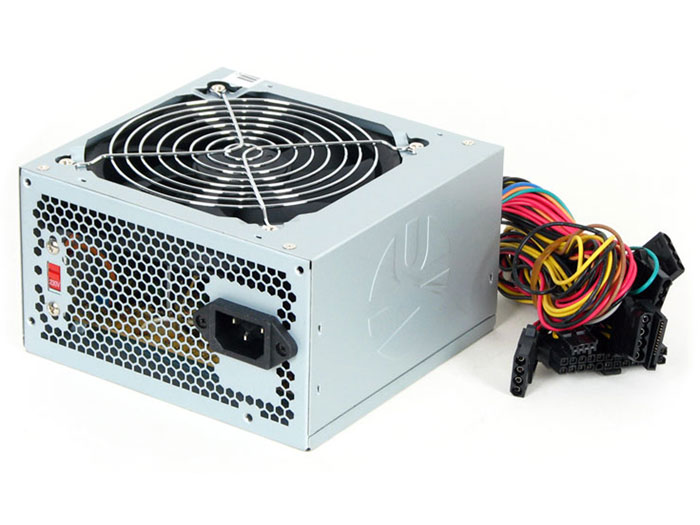
\includegraphics[scale=0.35]{fuente-alimentacion.jpg}
    \caption{Fuente de Alimentación}
\end{figure}

Desde la parte trasera de la fuente de alimentación podemos ver el conector para el cable de conexión a la fuente eléctrica y la rejilla de ventilación por la que su propio ventilador extrae el calor generado. Además, la parte trasera puede incluir, adicionalmente:

\begin{itemize}
    \item Un conector para la alimentación eléctrica del monitor.
    \item Un interruptor para el apaga total de la fuente de alimentación, que de otra forma permanece en estado de standby.
    \item Un selector para fijar la entrada de corriente alterna en 125 voltios o 220 voltios.
\end{itemize}

\subsection{Placas Bases}
La \textbf{Placa Base} es una tarjeta de circuito impreso donde se conectan el resto de componentes del computador. Contiene una serie de circuitos integrados entre los que se encuentra el \textbf{chipset}, que sirve como centro de conexión entre el procesador, la memoria RAM, los buses de expansión y otros dispositivos.

Su diseño debe cumplir con unos estándares basados en el \textbf{factor de forma}, que define algunas de las características físicas de esta, como por ejemplo:

\begin{itemize}
    \item La forma de la placa con sus dimensiones exactas (ancho y largo).
    \item La posición de los anclajes, es decir, donde se sitúan los tornillos para fijarla a la torre.
    \item Las áreas donde se sitúan algunos de sus componentes, como el zócalo del procesador, las ranuras de expansión y los conectores de la parte trasera.
    \item Las conexiones eléctricas de la fuente de alimentación: cantidad de conectores, forma, posición, etc...
\end{itemize}

En la siguiente imagen podemos ver una placa base con todos sus componentes.

\begin{figure}[ht]
    \centering
    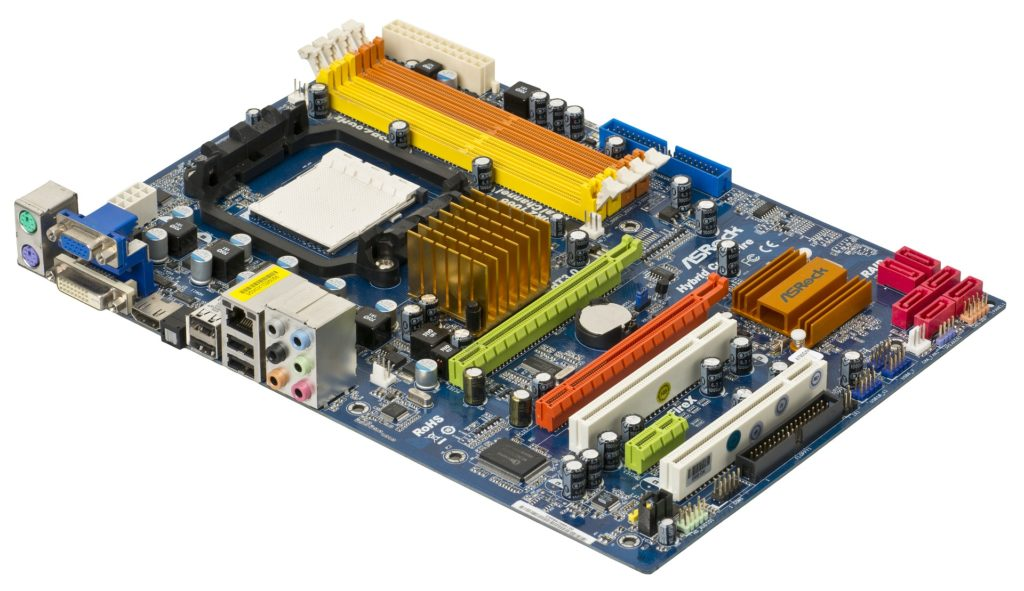
\includegraphics[scale=1]{placa-base.jpg}
    \caption{Placa base y sus componentes}
\end{figure}

Todos los conectores tienen conexión directa con alguno de los dos elementos principales del \textbf{chipset}, el \textbf{puente norte} o \textbf{northbridge} y el \textbf{puente sur} o \textbf{southbridge}. Se trata de dos circuitos integrados que con el tiempo han ido recogiendo en su diseño funcionalidades que antes fueron independientes. A saber:

\begin{itemize}
    \item \textbf{Northbridge}: se encarga de controlar funciones como las comunicaciones entre el procesador, la memoria y el sistema gráfico. Algunos modelos pueden incluir controladoras de vídeo, sonido y red.
    \item \textbf{Southbridge}: se encarga del control del resto de puertos internos y externos de la placa base.
\end{itemize}

\begin{figure}[ht]
    \centering
    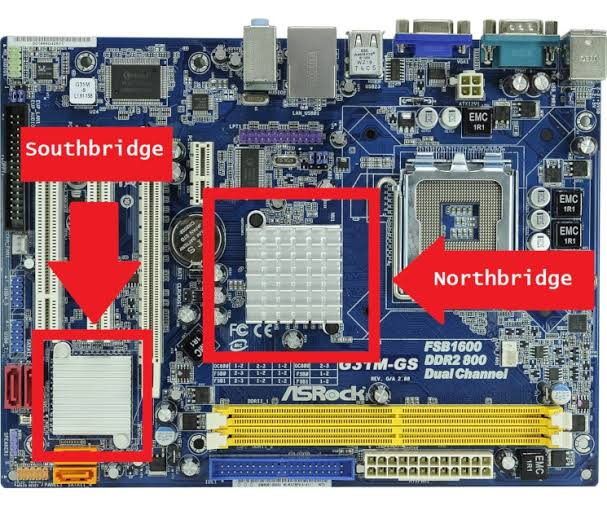
\includegraphics[scale=0.35]{puentes-placa.jpeg}
    \caption{Northbridge y Southbridge en una placa base}
\end{figure}

El chipset, por lo tanto, hace que la placa base funcione como un ``sistema nervioso'', que interconecta todos sus componentes por medio de diferentes buses, permitiendo la comunicación entre ellos.

La placa base también incluye un chip conocido como \textbf{\gls{BIOS}} con un software propio o \textbf{firmware}, que le permite realizar funcionalidades básicas, como reconocimiento y auto chequeo de los dispositivos instalados o gestión básica de vídeo y teclado. Es el software que se encarga del arranque del ordenador y que es independiente del sistema operativo.

En el \textbf{Anexo A.3} podemos encontrar una relación detallada de todos los componentes de una placa base, y que deberíamos de conocer.

\subsection{Procesadores}
El \textbf{procesador} es la parte más importante del computador ya que controla al resto de componentes. Se trata de un microchip compuesto de millones de microcomponentes recogidos en una cápsula, normalmente cerámica, que de la que salen una serie de patillas o contactos que hay que acoplar en el zócalo de la placa base.

Existen varios fabricantes de procesadores para ordenadores personales, siendo los mas potentes \textbf{AMD} e \textbf{Intel}, por ser los que más invierten en investigación y más productos sacan al mercado. En los siguientes enlaces podemos consultar los diferentes procesadores de estas compañías y su evolución.

\vspace{5ex}

\begin{itemize}
    \item \textbf{Procesadores AMD} - \url{http://www.configurarequipos.com/doc1043.html}
    \item \textbf{Procesadores Intel} - \url{http://www.configurarequipos.com/doc1051.html}
\end{itemize}

\begin{figure}[ht]
    \centering
    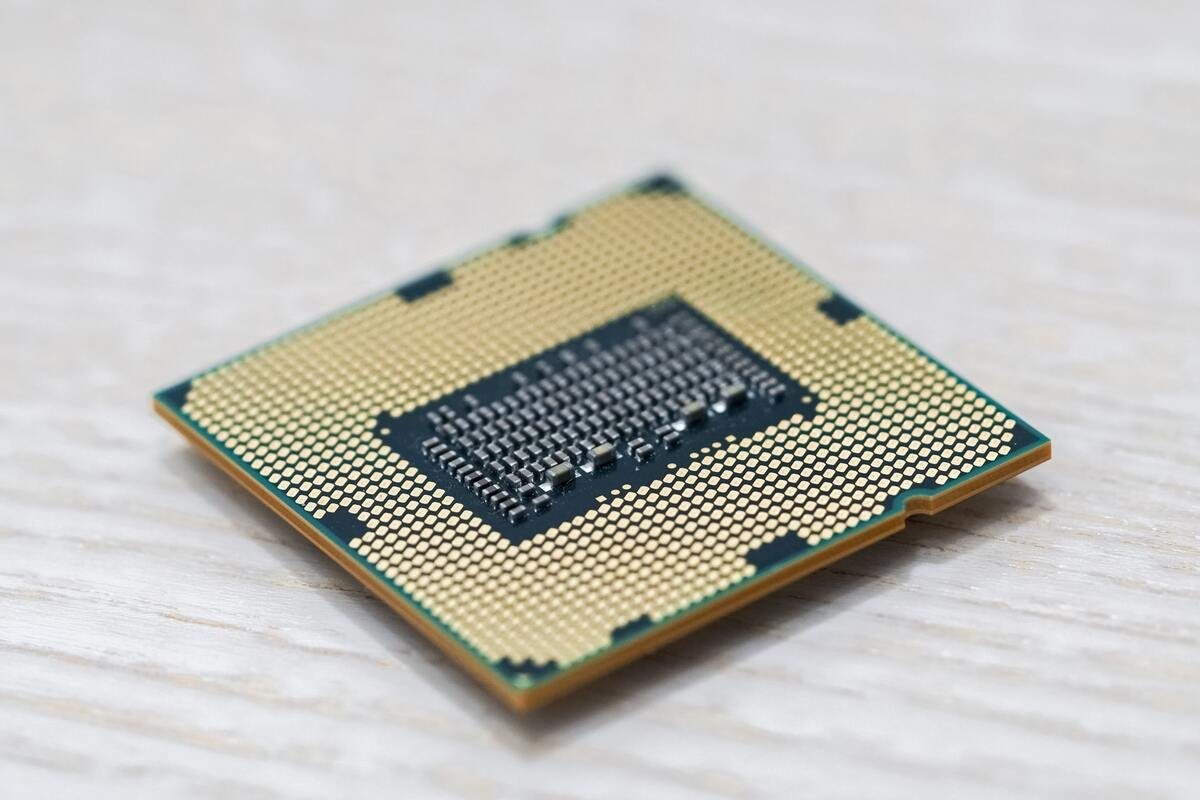
\includegraphics[scale=0.25]{cpu.jpg}
    \caption{Imagen de un procesador.}
\end{figure}

Hay diversas \textbf{características} que definen a un procesador:

\begin{itemize}
    \item \textbf{Velocidad de Cálculo}

    Es la velocidad de trabajo o frecuencia del reloj que me mide en \textbf{Hertzios}, o en alguno de sus submúltiplos. Con esta medida se especifica el número de ciclos por segundo, que esta relacionado con el número de operaciones por segundo que puede llevar a cabo el procesador. Se supone que cuantos mas hertzios tenga un procesador más operaciones podrá realizar por segundo y por lo tanto será más rápido.

    Hay que diferenciar entre al \textbf{velocidad interna} y la \textbf{velocidad externa} conocida como \textbf{Front Side Bus} (FSB), que es la velocidad de comunicación entre el procesador y la placa base. Esta medida es útil para comprar procesadores de un mismo fabricante, ya que ha iguales frecuencia de reloj pueden suponer diferentes velocidades de trabajo si comparamos procesadores de diferentes fabricantes.

    \item \textbf{Tecnología de Fabricación}

    La tecnología de fabricación, que se mide en \textbf{nanómetros}, es una medida utilizada para referirse al tamaño de los transistores que componen los procesadores. Cuanto menor sea el tamaño de los transistores, más cerca pueden colocarse unos de otros. Esto permite reducir la cantidad de energía eléctrica y por consiguiente reducir el calor generado por éstos durante el funcionamiento del microprocesador, que puede alcanzar mayores frecuencias de reloj. Actualmente se están fabricando procesadores entre 32 nm y 12 nm.

    \item \textbf{Tamaño y Nivel de la Memoria Caché}

    Es una memoria de gran velocidad utilizada para almacenar datos e instrucciones a los que el procesador debe de estar accediendo continuamente. La inclusión de una buena cantidad de memoria caché aumenta el rendimiento ya que permite reducir el número de accesos que se realizan a la memoria RAM, más lenta.

    Suele haber varios tipos de memoria caché que se \textbf{organizan por niveles}, creando una jerarquía basada en en la proximidad al núcleo del procesador, de forma que cuanto más cerca éste, trabajará a mayor velocidad, pero será de menor tamaño. La cache puede ser:

    \begin{itemize}
        \item \textbf{Caché de primer nivel o L1}: caché que esta integrada en el núcleo del procesador y trabaja a la misma velocidad. Su capacidad varía de un procesador a otro estando entre los 64KB y los 512KB. Suele estar dividida en dos parte, una dedicada a trabajar con los datos y otra con las instrucciones.

        \item \textbf{Caché de segundo nivel o L2 y tercer nivel o L3}: suelen estar también integradas en el procesador aunque no en su núcleo y sus tamaños pueden variar entre los 3 MB y los 6 MB.
    \end{itemize}

    \item \textbf{Número de Núcleos}

    Otra de la características de los procesadores actuales es el \textbf{número de núcleos} que se integra en la cápsula y que pueden trabajar de forma simultánea. Como se esta haciendo difícil, o poco rentable, incrementar la velocidad de funcionamiento de los nuevos procesadores para continuar aumentando su rendimiento, los fabricantes han aprovechado el alto grado de integración conseguido en la fabricación de estos para encapsular varios núcleos dentro de un mismo procesador. Actualmente podemos encontrar procesadores con un variable número de núcleos, desde 2 núcleos a 16, o incluso más.

    \item \textbf{Arquitectura}

    En relación al funcionamiento, cabe destacar que otra característica de los procesadores es su \textbf{arquitectura}, la cual puede ser de \textbf{32 bits} o \textbf{64 bits}, que son los tamaños más utilizados en la actualidad. Esta medida se refiere al tamaño de los registros que contiene el procesador, y por tanto, al tamaño de las instrucciones que puede procesar éste. De este tamaño, dependerá el resto de la arquitectura del resto de componentes del procesador, ya que tendrán que trabajar con el mismo número de bits.
\end{itemize}

Hay que tener en cuenta que la elección de un procesador \textbf{condiciona la elección} de la \textbf{placa base}, ya que debe incluir un chipset acorde para que se puedan aprovechar todas las características del procesador, así como un zócalo compatible en el que pueda instalarse.

Además, hay que tener en cuenta que los procesadores, durante su funcionamiento, generan una gran cantidad de calor, por lo que deberemos tener en cuenta la incorporación de algún \textbf{sistema de refrigeración} que ayude a lidiar con el este calor. Los disipadores, que suelen ser los más empleados, consisten en un elemento metálico (de aluminio o cobre), con mucha superficie de contacto con el aire, que absorba el calor del procesador disipándolo en el aire. Esta \textbf{disipación} puede ser de dos tipos:

\begin{itemize}
    \item \textbf{Disipación pasiva}: solo incluye el disipador, el elemento metálico ya mencionado.
    \item \textbf{Disipación activa}: además del disipador, incluye un ventilador acoplado al disipador que crea un flujo de aire ayudando a disipar el calor más rápidamente.
\end{itemize}

Además, existen alternativas como por ejemplo la \textbf{refrigeración líquida}, que extrae el calor del procesador y de otros componentes aprovechando su mayor conductividad, aunque tiene el inconveniente de tener que instalar circuitos cerrados para hacer pasar el líquido por las zonas a refrigerar además de necesitar un radiador externo para que el líquido se desprenda de su calor.

\subsection{Memorias RAM}
La \textbf{memoria de acceso aleatorio} o memoria RAM (Random Access Memory) es la memoria que necesita el procesador para ejecutar los programas. En ella busca las instrucciones y datos, además de almacenar los resultados de las operaciones realizadas.

Físicamente, las memorias RAM son pequeñas tarjetas de circuito impreso en la que se sueldan los chips de memoria, por una o ambas caras. Llevan en uno de sus cantos un conjunto de pines o contactos metálicos para insertarlas en los zócalos de la placa base.

\begin{figure}[ht]
    \centering
    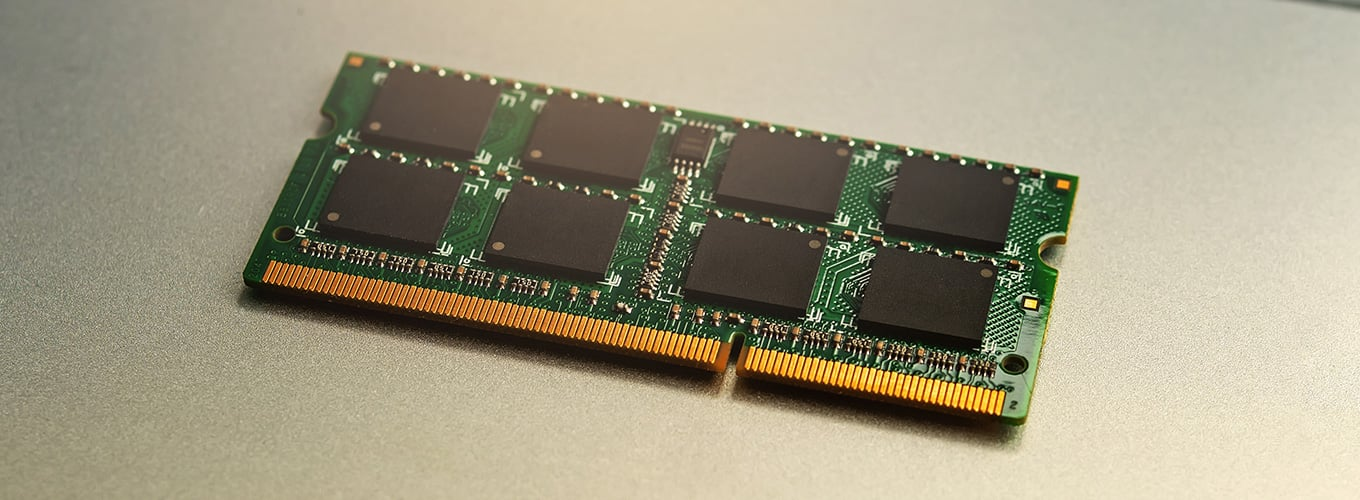
\includegraphics[scale=0.25]{ram.jpg}
    \caption{Módulo de memoria RAM tipo SO-DIMM}
\end{figure}

Actualmente podemos encontrar en el mercado diferentes tipos de módulos RAM, los más usados son de tipo \textbf{DDR} (Double Data Rate) o doble tasa de transferencia de datos que vienen integrados en tarjetas de memoria de tipo \textbf{DIMM} o \textbf{SO-DIMM}, usados en equipos de sobremesa y portátiles respectivamente.

Dentro de los módulos DDR, podemos encontrar diferentes versiones que determinarán el número de pines que poseen y donde se encuentra la muesca que les impide su colocación de forma incorrecta. Los principales tipos son:

\begin{itemize}
    \item \textbf{DDR}: son módulos RAM que usan memorias síncronas (SDRAM), en encapsulados de tipo DIMM, y que permiten hacer \textbf{dos transferencias simultáneas} en un mismo ciclo de reloj. Tienen \textbf{184 pines} en DIMM y \textbf{200 pines} en SO-DIMM.

    \item \textbf{DDR2}: trabajan al doble de frecuencia del reloj de la memoria, por lo que durante cada ciclo de reloj se realizan \textbf{cuatro trasferencias}. Tienen \textbf{240 pines} en DIMM y \textbf{200 pines} en SO-DIMM.

    \item \textbf{DDR3}: pueden realizar\textbf{ ocho transferencias }de datos por cada ciclo de reloj. Tiene \textbf{240 pines} en DIMM y \textbf{204 pines} en SO-DIMM.

    \item \textbf{DDR4}: no aumenta el número de transferencias de reloj, manteniéndose en 8, pero \textbf{aumenta la velocidad} incrementando la frecuencia de reloj. Además, tienen \textbf{mayor densidad} (mayor capacidad de datos) y menores requisitos de voltaje. Usan encapsulados DIMM con \textbf{288 pines} y SO-DIMM con \textbf{260 pines}.
\end{itemize}

\subsection{Tarjetas de Vídeo}
Una \textbf{tarjeta de vídeo} o \textbf{tarjeta gráfica}, es una tarjeta de expansión adicional, que adapta los daros enviados por el procesador al monitor o proyector para que el usuario pueda verlos representados.

La conexión de estos adaptadores a la placa base se realiza a través del bus \textbf{PCI Express x16}, ya que necesitan un bus rápido de comunicaciones. Hay modelos de  placas base y procesadores que integran en su circuitería un controlador gráfico de suficiente calidad para el uso normal del ordenador, pero que queda escaso de potencia de trabajo para aplicaciones que hagan uso intensivo de representación gráfica, como juegos o modelado 3D.

Para satisfacer la necesidades superiores gráficas de algunos programas, de diseño o juegos, hay placas base que ofrecen la posibilidad de conectar más de una tarjeta gráfica de modo que éstas puedan trabajar como una sola aumentando considerablemente su potencia.

\begin{figure}[ht]
    \centering
    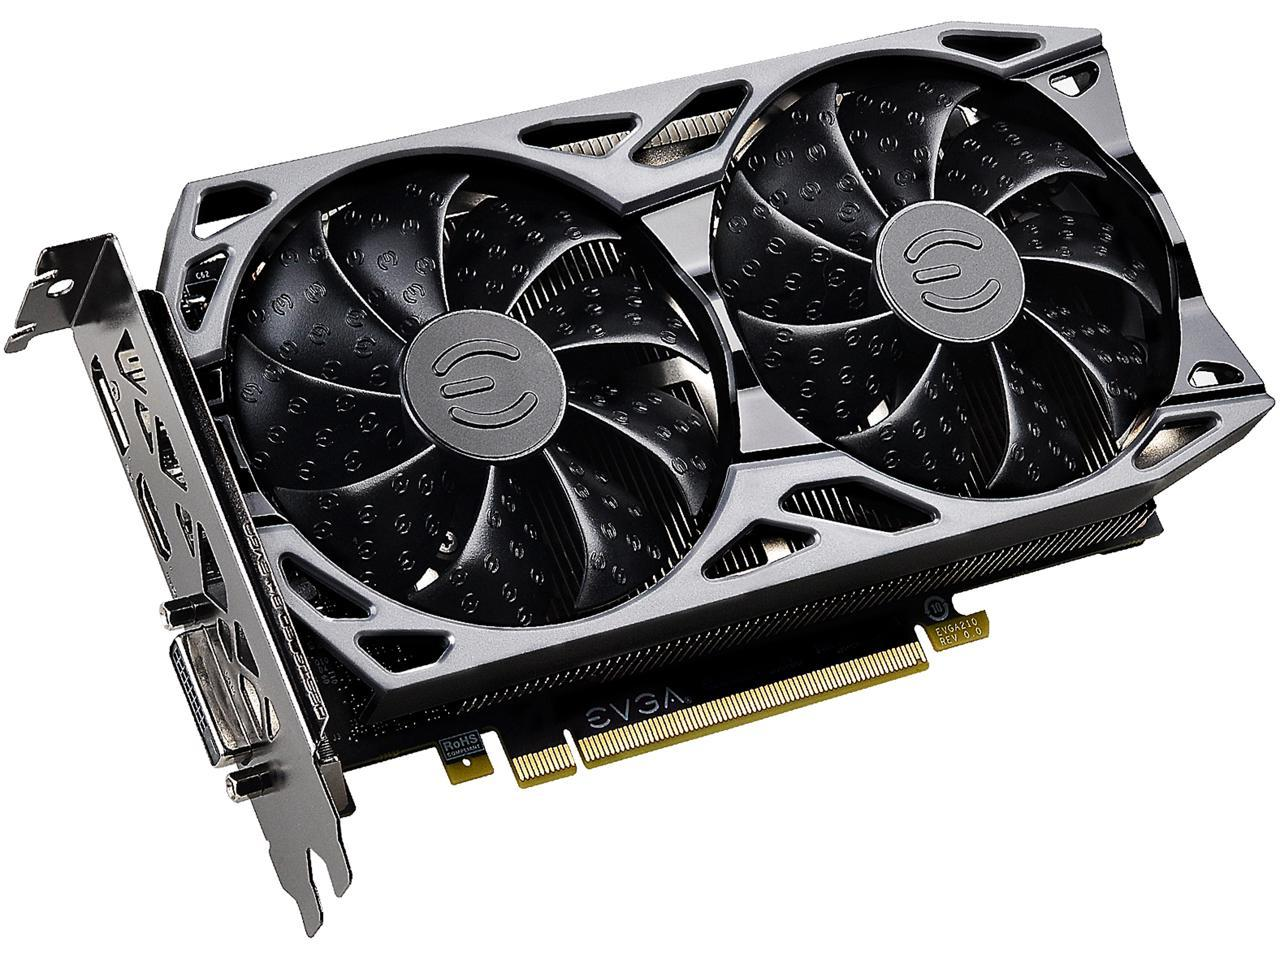
\includegraphics[scale=0.18]{gpu.jpg}
    \caption{Tarjeta gráfica con disipación activa}
\end{figure}

\newpage

Las tarjetas gráficas suelen tener, como mínimo, los siguientes elementos:

\begin{itemize}
    \item \textbf{La GPU}: es un procesador dedicado en exclusiva al tratamiento de gráficos, que libera al procesador de esta tarea. Necesita, al igual que el procesador, sistemas de refrigeración para disipar el calor.

    \item \textbf{La Memoria}: memoria que incorporan para el uso exclusivo de la propia tarjeta. Se llama memoria de vídeo y suele ser incluso más eficiente que la RAM del computador. Cuando la tarjeta gráfica esta integrada en la placa base o el procesador se suele reservar una parte de la memoria RAM para el uso de ésta.

    \item \textbf{EL RAMDAC}: es un conversor de imagen digital a analógica. Su función es transformar las señales para que pueden ser reproducidas en monitores analógicos. Este componente desaparece cuando todos los monitores sean digitales y reproduzcan directamente la señal digital.
\end{itemize}

Además de estos elementos, las tarjetas gráficas suelen incluir diferentes \textbf{conexiones} entre la tarjeta y ek monitor, siendo las más comunes son, \textbf{\gls{DVI}}, \textbf{\gls{S-Video}}, \textbf{\gls{SVGA}} y \textbf{\gls{HDMI}}.

Para ampliar más información sobre las tarjetas gráficas, podemos visitar su \href{https://es.wikipedia.org/wiki/Tarjeta_gr\%C3\%A1fica}{entrada en Wikipedia.}

\subsection{Tarjetas de Sonido}
Una \textbf{tarjeta de sonido} es una tarjeta de expansión que permite la entrada y salida de audio a través de sus conectores. Normalmente se inserta en una ranura \textbf{PCI}, aunque la mayoría de modelos de placa base vienen ya con una integrada. Las tarjetas de sonido incorporan conectores de tipo mini-jack que se necesitan para la conexión de equipos de sonido. Estos conectores tienen un código de colores que detallamos a continuación:

\begin{itemize}
    \item Entrada analógica para micrófono: \textbf{rosa}.
    \item Entrada analógica ``Line-In'': \textbf{azul}.
    \item Salida analógica estéreo para altavoces frontales: \textbf{verde}.
    \item Salida analógica para altavoces traseros: \textbf{negro}.
    \item Salida analógica para altavoces laterales: \textbf{plateado}.
    \item Salida digital SPDIF: \textbf{naranja}.
\end{itemize}

Además de estas conexiones, algunas tarjetas incluyen una

\begin{figure}[ht]
    \centering
    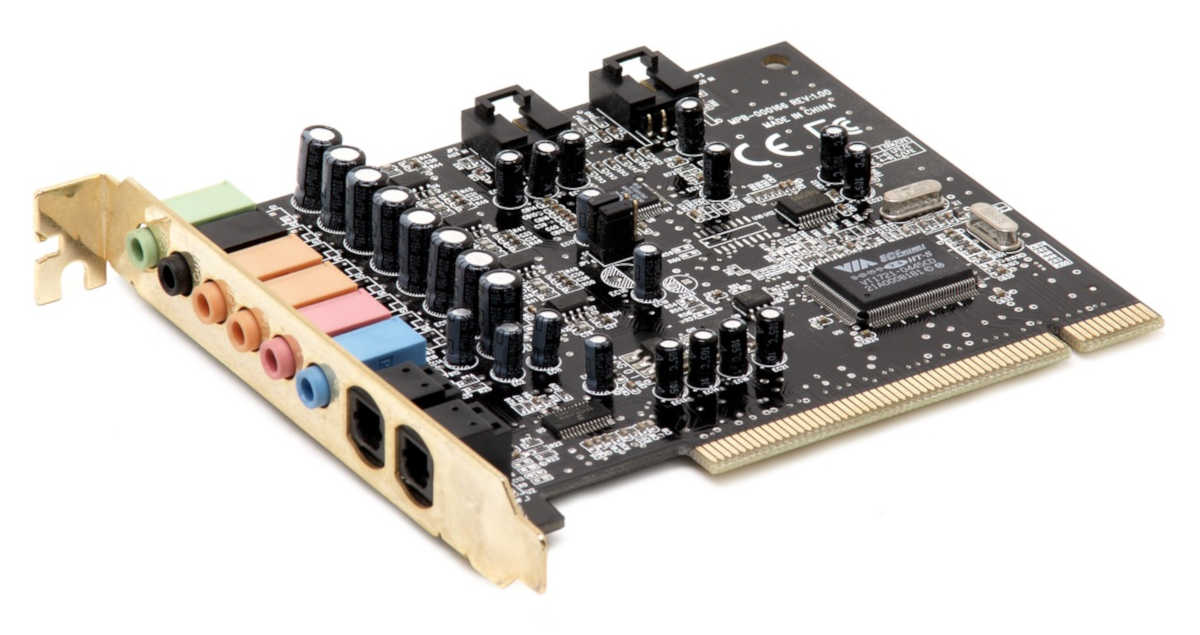
\includegraphics[scale=0.25]{tarjeta-sonido.jpg}
    \caption{Tarjeta de sonido}
\end{figure}

Las tarjetas de sonido necesitan tener varios componentes para poder procesar el sonido. Estos componentes son los siguientes:

\begin{itemize}
    \item \textbf{Circuito CAD} (Conversor Analógico-Digital): se encarga de transformar la señal analógica del sonido en su equivalente digital.
    \item \textbf{Circuito DAC} (Conversor Digital-Analógico): se encarga de transformar la señal digital en analógica de modo que pueda ser reproducida en unos altavoces.

    Para que la tarjeta de sonido pueda grabar y reproducir sonido al mismo tiempo ambos conversores, el CAD y el DAC, deben trabajar de forma independiente, lo que se conoce como \textbf{full-duplex}.

    \item \textbf{Circuito DSP} (Procesador de Señal Digital): se encarga de procesar el audio en su forma digital, realizando la compresión del audio cuando se graba y descomprimiendo cuando se reproduce. Además, por medio de algoritmos puede aplicar efectos acústicos  a los sonidos como coros, reverb, etc...

    \item \textbf{Sintetizador FM} (Modulación de Frecuencia): se encarga de generar sonido en formato \textbf{\gls{MIDI}} a partir de representaciones simbólicas de sus características.

    \item \textbf{Sintetizador por Tablas de Onda}: genera el sonido a partir de conjunto de muestras de sonido, de instrumentos reales, pregrabados en formato digital en una memoria ROM que incluye la propia tarjeta. El sintetizador para reproducir audio busca en las tablas que necesita en cada momento.

    \item \textbf{Mezclador}: tiene como finalidad recibir múltiples entradas, combinarlas adecuadamente, y enviarlas a las salidas.
\end{itemize}

Para obtener más información sobre las tarjetas de sonido, podemos visitar la \href{https://es.wikipedia.org/wiki/Tarjeta_de_sonido}{entrada en Wikipedia} referente a éstas.

\subsection{Dispositivos de Entrada}
Son todos aquellos \textbf{periféricos} que puede utilizar el usuario para \textbf{introducir información} al ordenador. Para ello será necesario que estén conectados a éste de alguna de las formas posibles. La mayoría de conexiones utilizadas, sobre todo en dispositivos de bajo consumo, reciben la alimentación necesaria a través del mismo conector, como por ejemplo, el teclado o el ratón. En cambio, otros dispositivos, debido a su alto consumo, necesitarán tener su propia fuente de alimentación, como por ejemplo, algunos escáneres. A continuación mostramos una lista con los dispositivos de entrada más comunes que nos podemos encontrar.

\begin{itemize}
    \item \textbf{Teclado}

    Es uno de los dispositivos de entrada más comunes, y casi imprescindibles, que utilizamos para \textbf{enviar información} al ordenador mediante la \textbf{pulsación de sus teclas}. Su modo de funcionamiento incluye que lo tecleado aparezca automáticamente en la pantalla, pudiendo así comprobar que se ha teclado de forma correcta.

    Se conecta al ordenador mediante un conector de tipo \textbf{PS/2} (o mini-din) a su conexión exclusiva, o por medio de conector \textbf{USB}. También los hay \textbf{inalámbricos} que necesitan dos terminales con emisor y receptor, uno de ellos en el propio teclado y otro que debe estar conectado al ordenador mediante el puerto PS/2 o USB. Además, entre los inalámbricos nos encontramos a los que usan el protocolo \textbf{bluetooth}, pudiendo aprovechar los emisores ya incorporados al ordenador.

    \begin{figure}[ht]
        \centering
        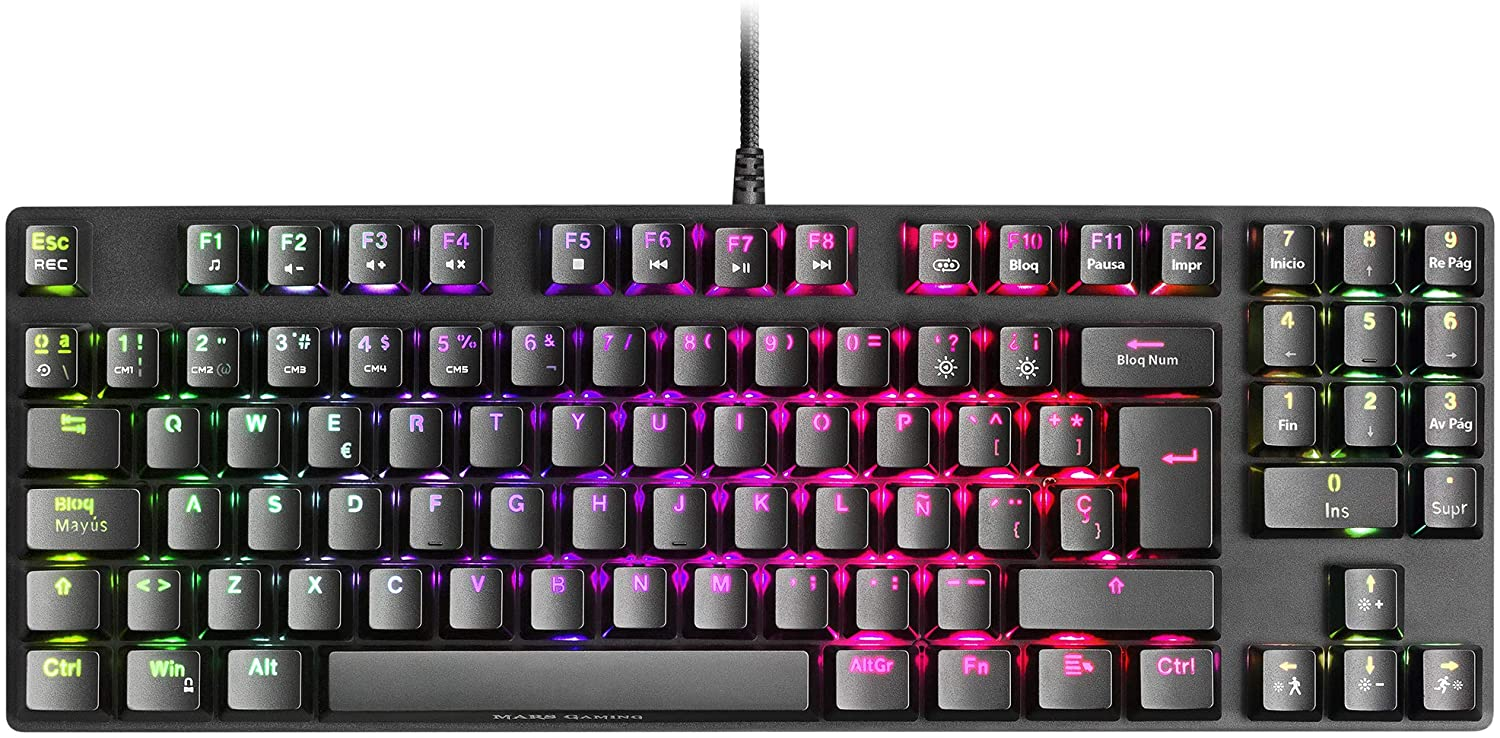
\includegraphics[scale=0.15]{teclado.jpg}
        \caption{Teclado estándar}
    \end{figure}

    \item \textbf{Ratón}

    El teclado es un dispositivo que al \textbf{ser desplazado} por una superficie plana, \textbf{mueve} sobre la pantalla un \textbf{cursor} que lo representa reflejando sus movimientos.

    Dependiendo del modelo, el ratón puede tener dos o más botones, incluso varias ruedas de desplazamiento, que permiten dar diversas órdenes en función del botón pulsado y del número de pulsaciones.  El cursor, que suele tener forma de flechas, se usa para \textbf{señalar diferentes objetos gráficos} en la \textbf{pantalla}.

    Se conecta al ordenador mediante un puerto PS/2 o USB, aunque al igual que con los teclados, podemos encontrarlos inalámbricos.

    \vspace{4ex}

    \begin{figure}[ht]
        \centering
        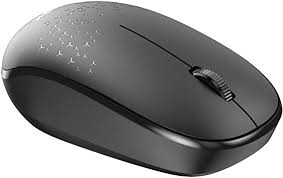
\includegraphics[scale=0.50]{raton.jpg}
        \caption{Ratón con 2 botones y rueda}
    \end{figure}


    \item \textbf{Joystick}

    El joystick o palanca es un periférico similar al ratón en cuanto \textbf{transmite los movimientos} que realicemos con él al ordenador. Se  utiliza sobre todo en juegos para dirigir el movimiento de personajes o vehículos.

    Suele conectar el ordenador mediante un puerto USB. Algunas tarjetas de sonido traen un conector específico para él.

    \begin{figure}[ht]
        \centering
        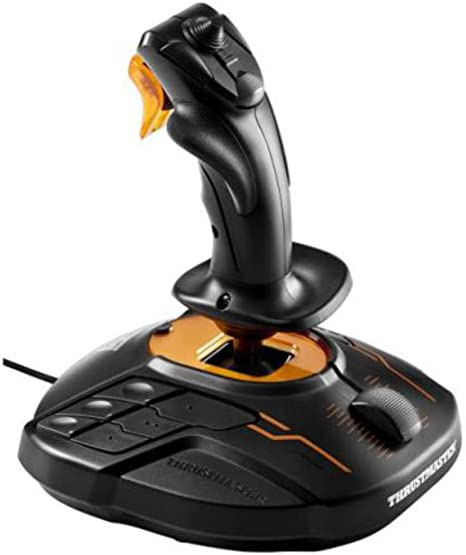
\includegraphics[scale=0.25]{joystick.jpg}
        \caption{Joystick estándar}
    \end{figure}

    \item \textbf{Escáner}

    Se utiliza para \textbf{explorar objetos} y obtener su \textbf{representación digital}. El proceso de digitalización consiste en tomar información de cada punto de la superficie del objeto y representarlos con valores binarios para generar un duplicado digital que pueda procesador el ordenador.

    Utiliza una conexión USB para conectarse al ordenador y algunos necesitan toma de corriente eléctrica para su propia alimentación. Además, podemos encontrar diferentes modelos de escáner,  como de sobremesa, de rodillo, de tambor, etc...

    \begin{figure}[ht]
        \centering
        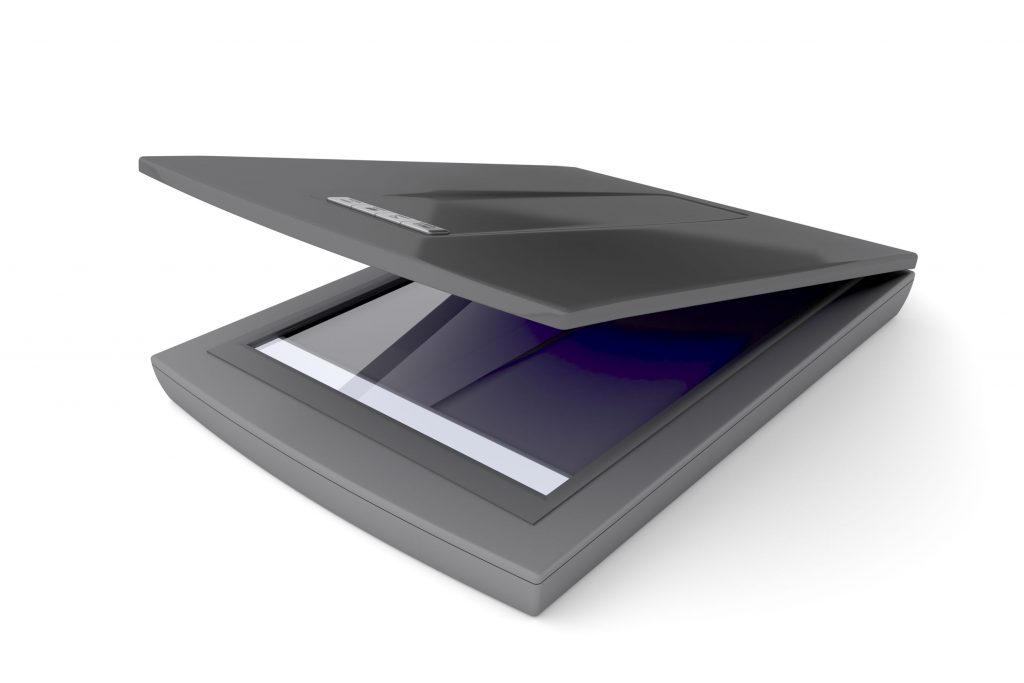
\includegraphics[scale=0.30]{escaner.jpg}
        \caption{Escáner de sobremesa}
    \end{figure}

    \item \textbf{Lectores de Código de Barras}

    Podemos encontrar tanto lectores de mano como fijos. Ambos, son \textbf{escáneres especializados} en la tarea de leer e interpretar códigos de barras. No se utilizan para obtener la representación digital del código de barras, sino el valor numérico que representan. Según el modelo, pueden conectarse al ordenador por USB, puerto de serie, Wi-Fi, bluetooth e incluso al puerto del teclado medio de un adaptador.

     \begin{figure}[ht]
        \centering
        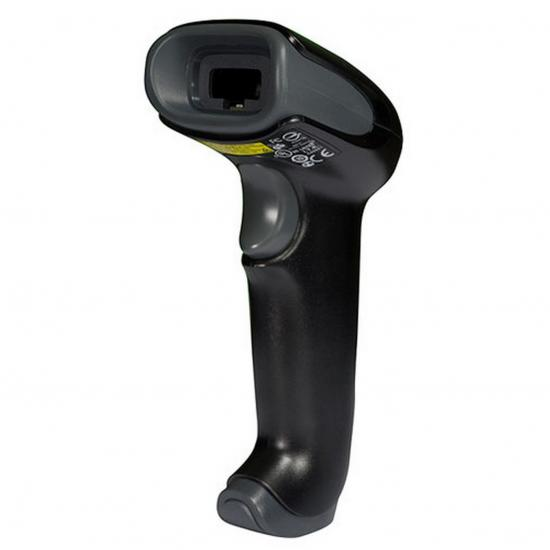
\includegraphics[scale=0.25]{lector-barras.jpg}
        \caption{Lector de código de barras de mano}
    \end{figure}

    \item \textbf{Tableta Gráfica o Digitalizadora}

    Este periférico permite la \textbf{introducción de dibujos o gráficos} dibujados \textbf{a mano} como si se hiciera con papel y lápiz. Se trata de una tablilla plana donde el usuario escribe utilizan el lápiz que suele acompañarla, aunque los trazos aparecen en la pantalla en vez de en la tableta.

    Algunas tabletas tiene delimitadas zonas de actuación que al ser pulsadas con el lápiz funcionan como botones e incluso pueden usarse como un ratón de gran precisión ya que permite apuntar y seleccionar los objetos que se encuentran en pantalla. Las tabletas actuales, suelen conectarse mediante el puerto USB, aunque hay modelos que lo hacen mediante bluetooth o Wi-Fi.

     \vspace{4ex}

    \begin{figure}[ht]
        \centering
        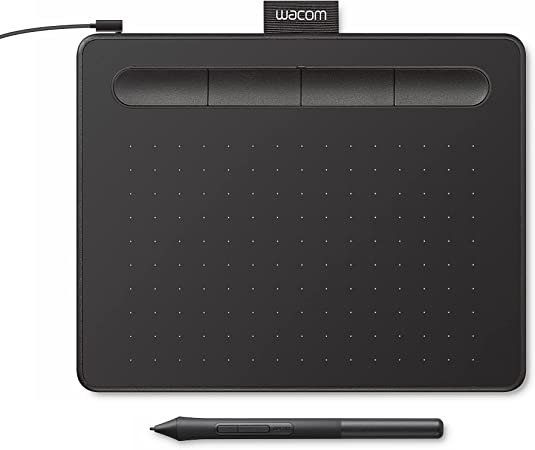
\includegraphics[scale=0.32]{tableta-digi.jpg}
        \caption{Tableta digitalizadora y su lápiz}
    \end{figure}

    \item  \textbf{Micrófono}

    Este dispositivo permite la \textbf{introducción de sonidos en el ordenador}, como música o la propia voz. Su conexión se realiza a través de un conector de tipo mini jack, incluido en la tarjeta de sonido que debe estar incluida en el ordenador para que pueda ser utilizado. También hay otros micrófonos que se conectan directamente a un puerto USB, comportándose como un dispositivo de grabación sin necesidad de tarjeta de sonido.

    \vspace{4ex}

    \begin{figure}[ht]
        \centering
        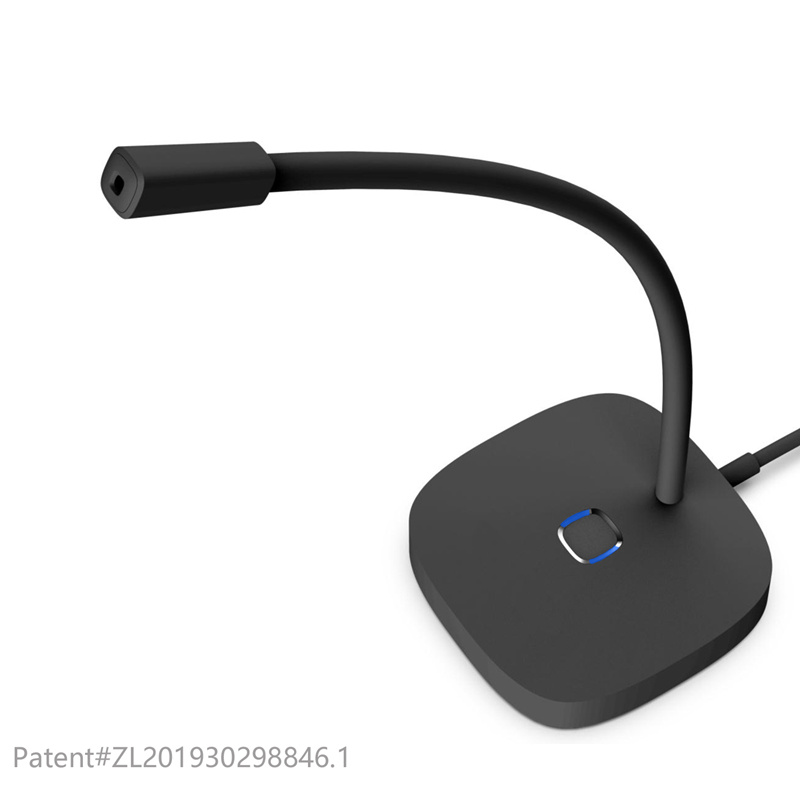
\includegraphics[scale=0.55]{microfono.jpg}
        \caption{Micrófono de ordenador}
    \end{figure}

    \item \textbf{Cámara Digital}

    Dispositivo cuya finalidad es \textbf{captar imágenes} y \textbf{codificarlas en binario} para que puedan ser procesadas por el ordenador. Estas capturas pueden ser guardadas como imágenes estáticas o como imágenes en movimiento. En la actualidad, distinguimos principalmente dos tipos de cámaras, las cámaras web, que necesitan un ordenador para transmitir la información, al que se conectan mediante USB, o las llamadas cámaras de red, que se conectan a un punto de la red , de forma inalámbrica o mediante cable.

    La mayoría de los actuales portátiles ya llevan incluida una cámara web en la carcasa. También las cámaras fotográficas y de vídeo digitales, que aunque trabajan de forma independiente, pueden conectarse al ordenador mediante USB o fireware, para descargar en él sus capturas.

     \begin{figure}[ht]
        \centering
        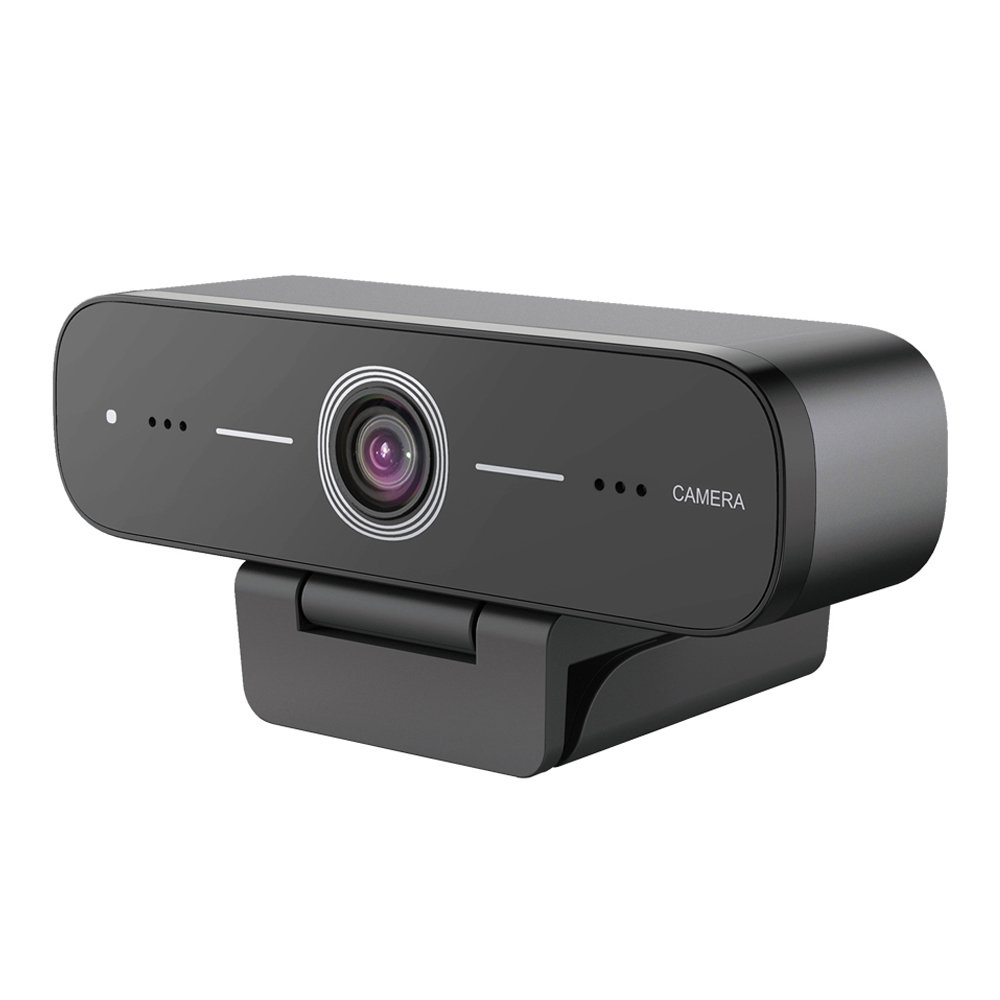
\includegraphics[scale=0.15]{webcam.jpeg}
        \caption{Webcam estándar}
    \end{figure}
\end{itemize}

Como vemos, la cantidad de periféricos que podemos conectar al ordenador es enorme. Y éstos son solo los más empleados, hay otros muchos dispositivos que aunque son menos comunes también se emplean como dispositivos de entrada, como pueden ser lectores magnéticos (de tarjetas, por ejemplo), lectores de huellas digitales, etc...

\subsection{Dispositivos de Salida}
Después de ver los dispositivos de entrada, vamos a ver los de salida. Éstos son todos aquellos periféricos que puede utilizar el usuario para obtener información del ordenador. Juntos con los dispositivos de entrada, son el conjunto de elementos que permiten la comunicación persona-ordenador.

A continuación, mostramos una lista con los dispositivos de salida más empleados:

\vspace{3ex}
\begin{itemize}
    \item \textbf{El Monitor}

    El monitor es un dispositivo que \textbf{muestra la interfaz} proporcionada por lo \textbf{programas} para que interactuemos con ellos. Mediante esta interfaz visual podemos hacer que se ejecuten programas al pulsar en sus iconos y responder a las peticiones que nos hagan estos, así como \textbf{ver los resultados} de su ejecución. También nos permite ver los datos mientras que los introducimos desde el teclado o los movimientos del puntero cuando usamos el ratón. En la actualidad, existen diferentes tipos de monitores según la tecnología que emplean para representar las imágenes. Los mas comunes son los siguientes:

    \begin{itemize}
        \item \textbf{Monitores CRT}: son monitores que usan un tubo de rayos catódicos para dibujar las imágenes en la pantalla. Están cayendo en desuso debido a su gran tamaño.

        \item \textbf{Monitores LCD}: son monitores que usan un pantalla de cristal líquido para representar las imágenes. Dentro de estos podemos encontrar los LCD de matriz activa, mas conocidos como \textbf{TFT} (Thin Film Transistor), siendo muy utilizados en informática debido a su gran calidad de imagen.

        \item \textbf{Monitores LED}: son monitores que usan leds para representar las imágenes. En la actualidad son cada vez más utilizados debido a su bajo consumo.
    \end{itemize}

     \begin{figure}[ht]
        \centering
        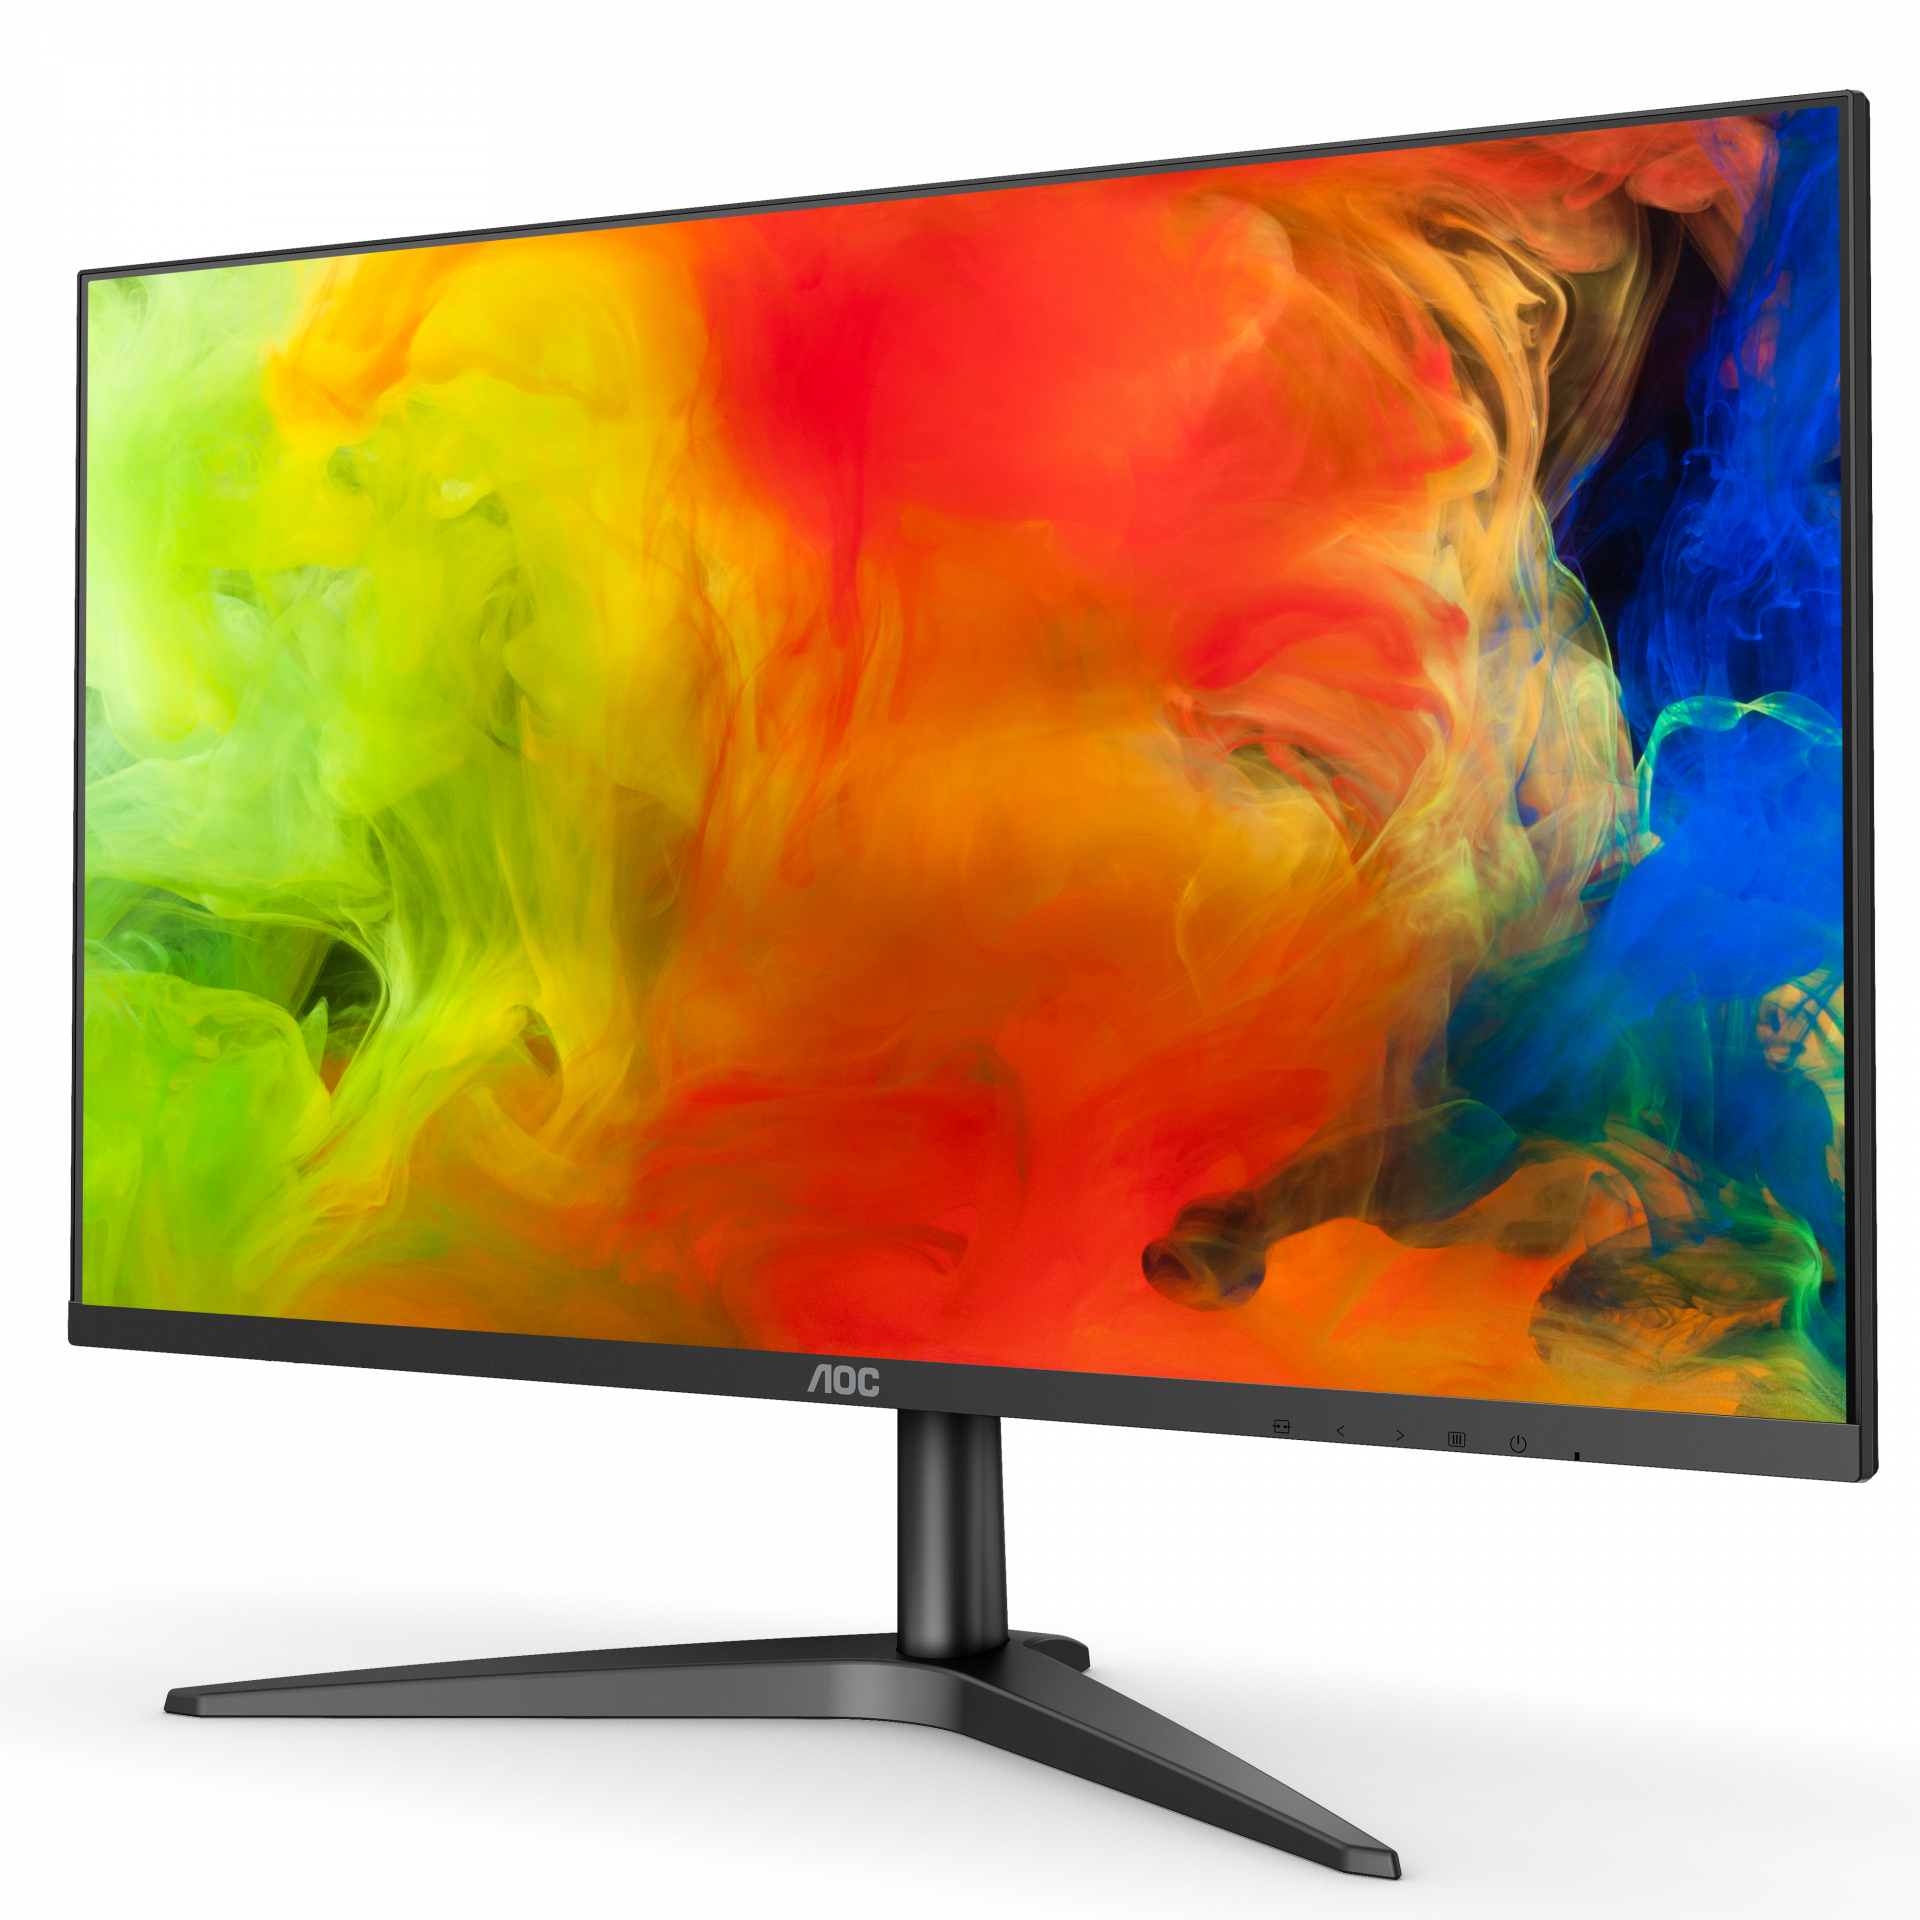
\includegraphics[scale=0.13]{monitor.png}
        \caption{Monitor de tipo LED}
    \end{figure}

    Además de clasificarlos por la tecnología que emplean para representar las imágenes, los monitores tienen otras características que determinan su calidad y la calidad de imagen que pueden representar. Las principales de estas características son las estas:

    \begin{itemize}
        \item \textbf{Tamaño del Monitor}: expresa la longitud de su diagonal medida en pulgadas. Un LCD normal suele tener 17 pulgadas o más, por ejemplo.

        \item \textbf{Tamaño del Punto}: esta medida es usada para conocer el tamaño entre dos puntos del mismo color en la pantalla. Cuanto menor sea el tamaño del punto mejor será su definición, ya que al estar más juntos los puntos que forman las imágenes mayor nitidez tendrán éstas. En estándar mas usado es una tamaño de punto de 0.24 mm.

        \item \textbf{Resolución}: la resolución indica el número total de puntos que puede representar el monitor y se expresa como el producto de dos números, ancho x alto. Así, un monitor que tenga una resolución de 1024x768 puede representar 1024 líneas en vertical y 768 en horizontal.
    \end{itemize}

    En cuanto a la conexión de los monitores al ordenador, ésta puede ser tipo analógico (SVGA o RGB), que era lo común en los monitores CRT, pero desde que se están imponiendo los monitores digitales, ya no es necesario convertir la señal de salida de las tarjetas gráficas en analógica y la conexión se realiza mediante conectores digitales (DVI o HDMI).

    \item \textbf{Los Altavoces}

    Los altavoces son dispositivos de salida que \textbf{permiten reproducir sonidos}, voces, música, etc.., a través de una tarjeta de sonido a la que deben estar conectados. Pueden sustituirse por unos auriculares. También hay altavoces que se conectan mediante un puerto USB y no necesitan estar conectados a una tarjeta de sonido.

    \begin{figure}[ht]
        \centering
        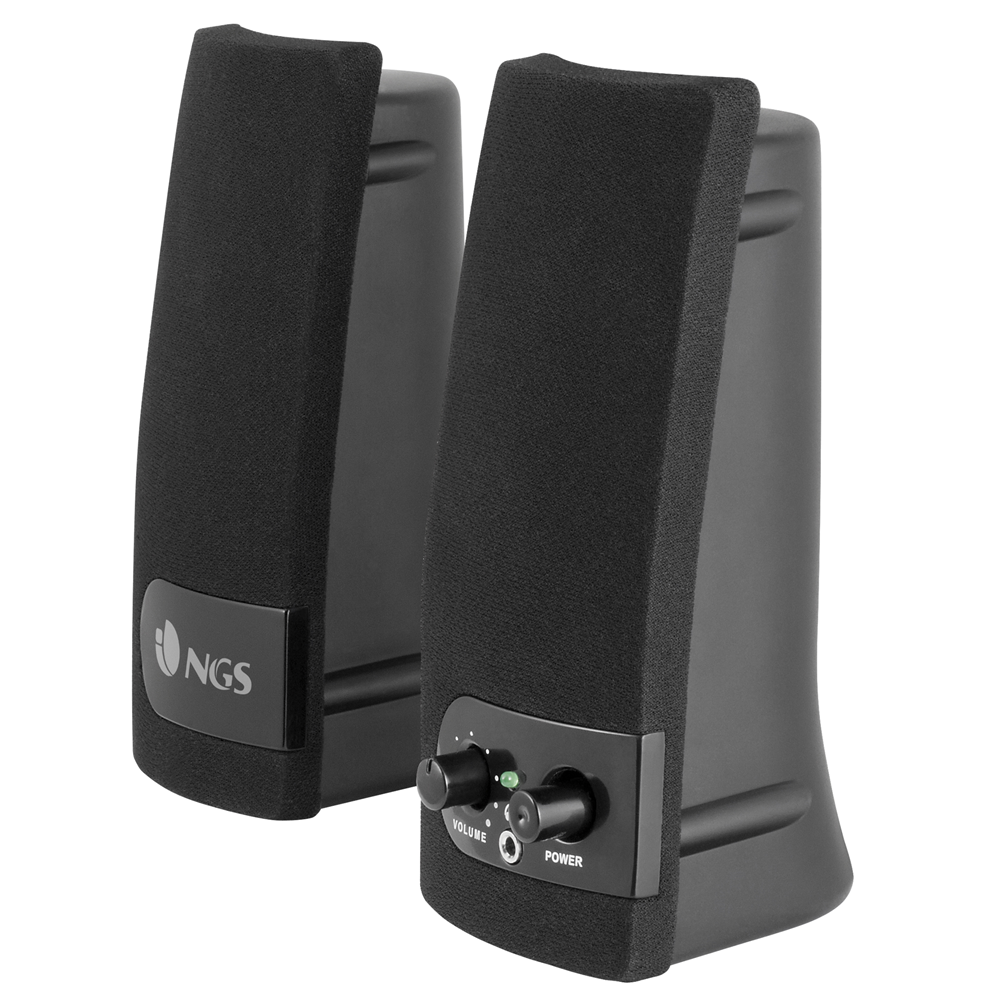
\includegraphics[scale=0.15]{altavoces.png}
        \caption{Altavoces para un PC}
    \end{figure}

    \item \textbf{La Impresora}

    Una impresora es un dispositivo de salida que \textbf{permite plasmar sobre la papel }la información proceden del ordenador. Se puede considerar como uno de los periféricos más antiguos, incluso más que el teclado o el monitor. Tienen un puerto propio de conexión, el puerto paralelo, aunque esta cayendo en desuso en favor de conexiones USB o de conexiones de red, ya sea inalámbrica o por cable.

    Pueden estar dedicadas a un solo ordenador o compartidas por mucho, y pueden ser dispositivos únicos o multifunción, cuando van unidos en la misma carcasa a un escáner o un fax. Necesitan de un cable de alimentación conectado a la red para abastecerse de energía.

    \begin{figure}[ht]
        \centering
        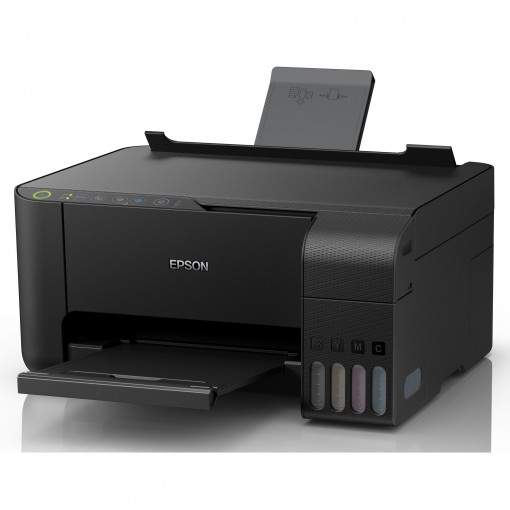
\includegraphics[scale=0.30]{impresora.jpg}
        \caption{Impresora multifunción}
    \end{figure}

    \item \textbf{El Plóter}

    El plóter, también llamado trazador gráfico, es un periférico diseñado para imprimir diseños de grandes dimensiones y con gran calidad. Muchos modelos permiten el uso de papel de gran ancho para la impresión de mapas, carteles, planos, patrones a tamaño real, etc...

    Una variedad de plóter son las cortadoras industriales, usadas para cortar patrones de confección o para cortar piezas metálicas u otros materiales como el metacrilato. En ellas, se sustituye la tinta por un láser de corte.

    Los plóter actuales se conectan a la red mediante un enlace ethernet y pueden ser compartidos por varios computadores.

    \begin{figure}[ht]
        \centering
        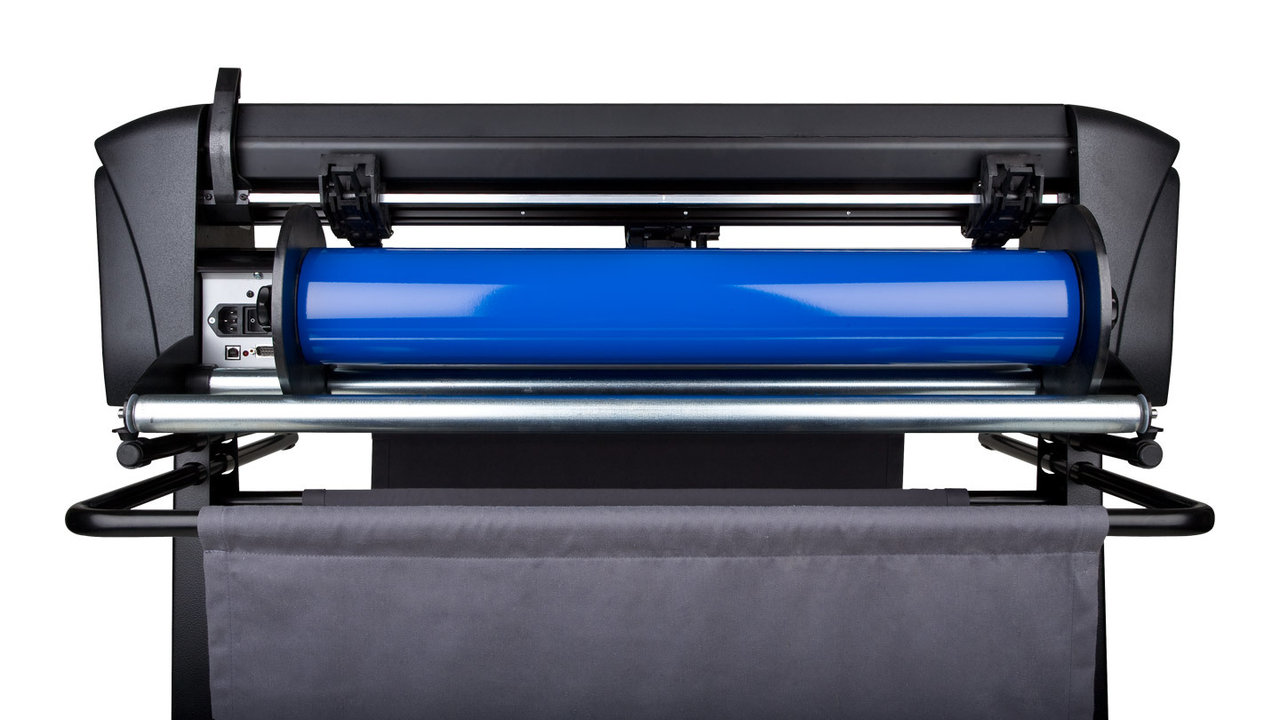
\includegraphics[scale=0.15]{ploter.jpg}
        \caption{Plóter de corte}
    \end{figure}
\end{itemize}

\subsection{Dispositivos de Entrada/Salida}
Los dispositivos de entrada/salida son aquellos que nos permiten tanto introducir la información en el computador como visualizarla o almacenarla, aunando las características de los dispositivos vistos en los dos puntos anteriores.

Basándonos en lo que hacen con la información que maneja, podemos clasificarlos en \textbf{dispositivos que almacenan} la \textbf{información} y \textbf{dispositivos que no la almacenan}. Así, los dispositivos de entrada/salida más empleados son los siguientes:

\subsubsection{Dispositivos de E/S sin Almacenamiento}

Estos dispositivos se limitan a transmitir la información, ya sean hacia el ordenador por parte del usuario, desde el ordenador al usuario o entre distintos ordenadores. Los más comunes son:

\begin{itemize}
    \item \textbf{Pantalla Táctil o Touch Screen}

    Estos dispositivos son pantallas, que ya de por si son dispositivos de salida, que además incorporan un mecanismo que le permite capturar información cuando algún elemento hace contacto sobre su superficie, como un dispositivo apuntador o un dedo. Deben trabajar conjuntamente con algún software que asocie las pulsaciones con acciones concretas.

    Para detectar el punto de contacto en la pantalla se suelen emplear diferentes tecnologías, siendo las más comunes:

    \begin{itemize}
        \item \textbf{Pantallas resistivas}: se sitúa sobre la pantalla una cuadrícula eléctrica en dos plano de modo que al ejercer presión un filamento horizontal entra en contacto con otro vertical, detectándose así el área presionada.
        \item \textbf{Pantallas por infrarrojos}: consiste en una matriz de sensores y emisores infrarrojos horizontales y verticales. En cada eje los receptores están en el lado opuesto de los emisores, de forma que al tocar en algún punto de la pantalla el haz infrarrojo se interrumpe, permitiendo de esta forma localizar el punto presionado.
        \item \textbf{Pantallas de pulso acústico}: utilizan cuatro transductores piezoeléctricos situados a cada lado de la pantalla que convierte la energía mecánica de contacto en una señal electrónica. Esta señal se convierte en una onda de sonido y se compara con la plantilla de sonidos que ya se tiene en cada posición de la pantalla.
    \end{itemize}

    \begin{figure}[ht]
        \centering
        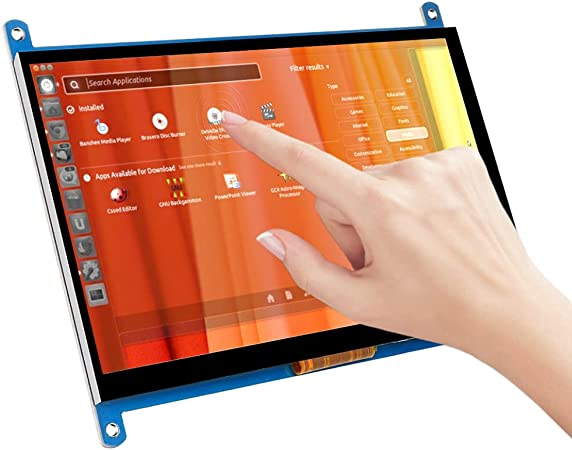
\includegraphics[scale=0.30]{touch.jpg}
        \caption{Pantalla de tipo Touch Screen}
    \end{figure}

    \item \textbf{Módem}

    El módem sirve para conectar un ordenador a otro a través de una red telefónica básica. Los ordenadores han de convertir sus datos binarios en la señal sonora de telefonía. Para ello, se convierte cada 1 en una frecuencia determinada y cada 0 en otra. En ordenador receptor debe descodificar esta señal y convertirla de nuevo en código binario. De estas conversiones, se encarga el modulador-demodulador del módem.

    Estos módem han quedado obsoletos en favor de dispositivos que transmiten utilizando la tecnología ADSL o mediante cable de fibra óptica.

    \begin{figure}[ht]
        \centering
        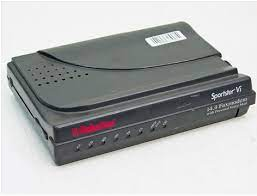
\includegraphics[scale=0.75]{modem.jpeg}
        \caption{Módem estándar}
    \end{figure}

    \item \textbf{Tarjeta de Red}

    Las tarjetas de red, son dispositivos que permite la conexión de ordenadores mediante una red local y la conexión de estos a internet ya sea mediante ADSL o cable. Pueden ser cableadas (ethernet) o inalámbricas (Wi-Fi) y la mayoría de ordenadores de la actualidad suelen traer ya una incorporada.
\end{itemize}

\begin{figure}[ht]
    \centering
    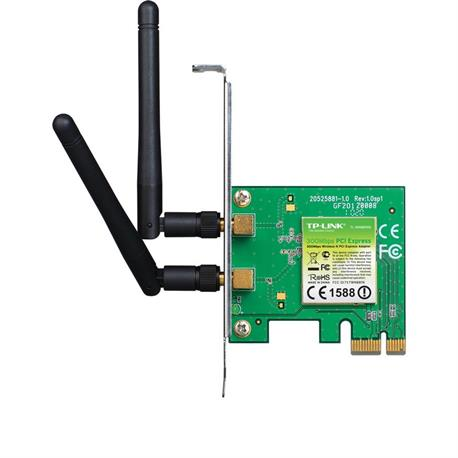
\includegraphics[scale=0.45]{tarjeta-wifi.jpg}
    \caption{Tarjeta de red inalámbrica}
\end{figure}

\subsubsection{Dispositivos de Almacenamiento Masivo}

Los dispositivos de almacenamiento son aquellos pueden almacenar la información de forma permanente sin necesidad de electricidad para mantenerla. Se les llama de \textbf{almacenamiento masivo} porque pueden guardar grandes cantidades de información. Se les conoce también como \textbf{memoria secundaria} o \textit{unidades de almacenamiento} y permiten que la información almacenada sea pueda ser utilizada cuando sea necesario y cuantas veces se precise. La información que guardan se almacena en formato binario.

Algunos dispositivos se bastan de si mismos para el almacenamiento de la información, como los discos duros, mientras que otros necesitan de un soporte de información para almacenarla, como los CD-ROMs o los DVDs.

El \textbf{soporte de información} es cualquier medio físico destinado a registrar la información de forma magnética, óptica o mediante cualquier otro método, siempre de forma permanente. Tienen la característica de ser intercambiables ya que pueden ser usados en cualquier otra unidad compatible de cualquier otro ordenador. Estos soporte suelen ser CD-ROMs, DVDs, cintas magnéticas, tarjetas de memoria, etc...

Los soporte de información los podemos clasificar según la forma de acceso a la información en:
\begin{itemize}
    \item \textbf{Secuenciales}: son aquellos en los que la información se accede de forma secuencial, teniendo que recorrer todos los elementos anteriores para obtener un elemento concreto. Suelen ser las cintas DAT o cualquier otro tipo de cinta. Se suelen emplear para backups o copias de seguridad.
    \item \textbf{Directos}: son aquellos en los que el acceso a la información se hace de forma inmediata sin tener que pasar por otra información anterior. Algunos ejemplos son discos duros, DVDs, etc...
\end{itemize}

Los principales tipos de dispositivos de almacenamiento, tanto secuencial como directos, son los siguientes:

\begin{itemize}
    \item \textbf{Lectores de Cintas Magnéticas}

    Las \textbf{cintas magnéticas} para el almacenamiento de datos vienen usando desde la segunda generación de ordenadores. Desde entonces han ido evolucionando en su forma y composición, aumentando su densidad de grabado, paralelamente a como lo han hecho las lectoras/grabadoras. Acceden a la información de \textbf{forma secuencial}.

    Las unidades lectoras deben tener en su interior unos mecanismos que permitan mover la cinta por delante de su cabeza de lectura y escritura, para poder registrar o leer en ella la información de forma magnética.

    Su principal ventaja es su gran capacidad, siendo hoy en día el medio más económico para realizar copias de seguridad de grandes volúmenes de información, proceso para el que su forma de acceso secuencial no es una desventaja.

    \begin{figure}[ht]
        \centering
        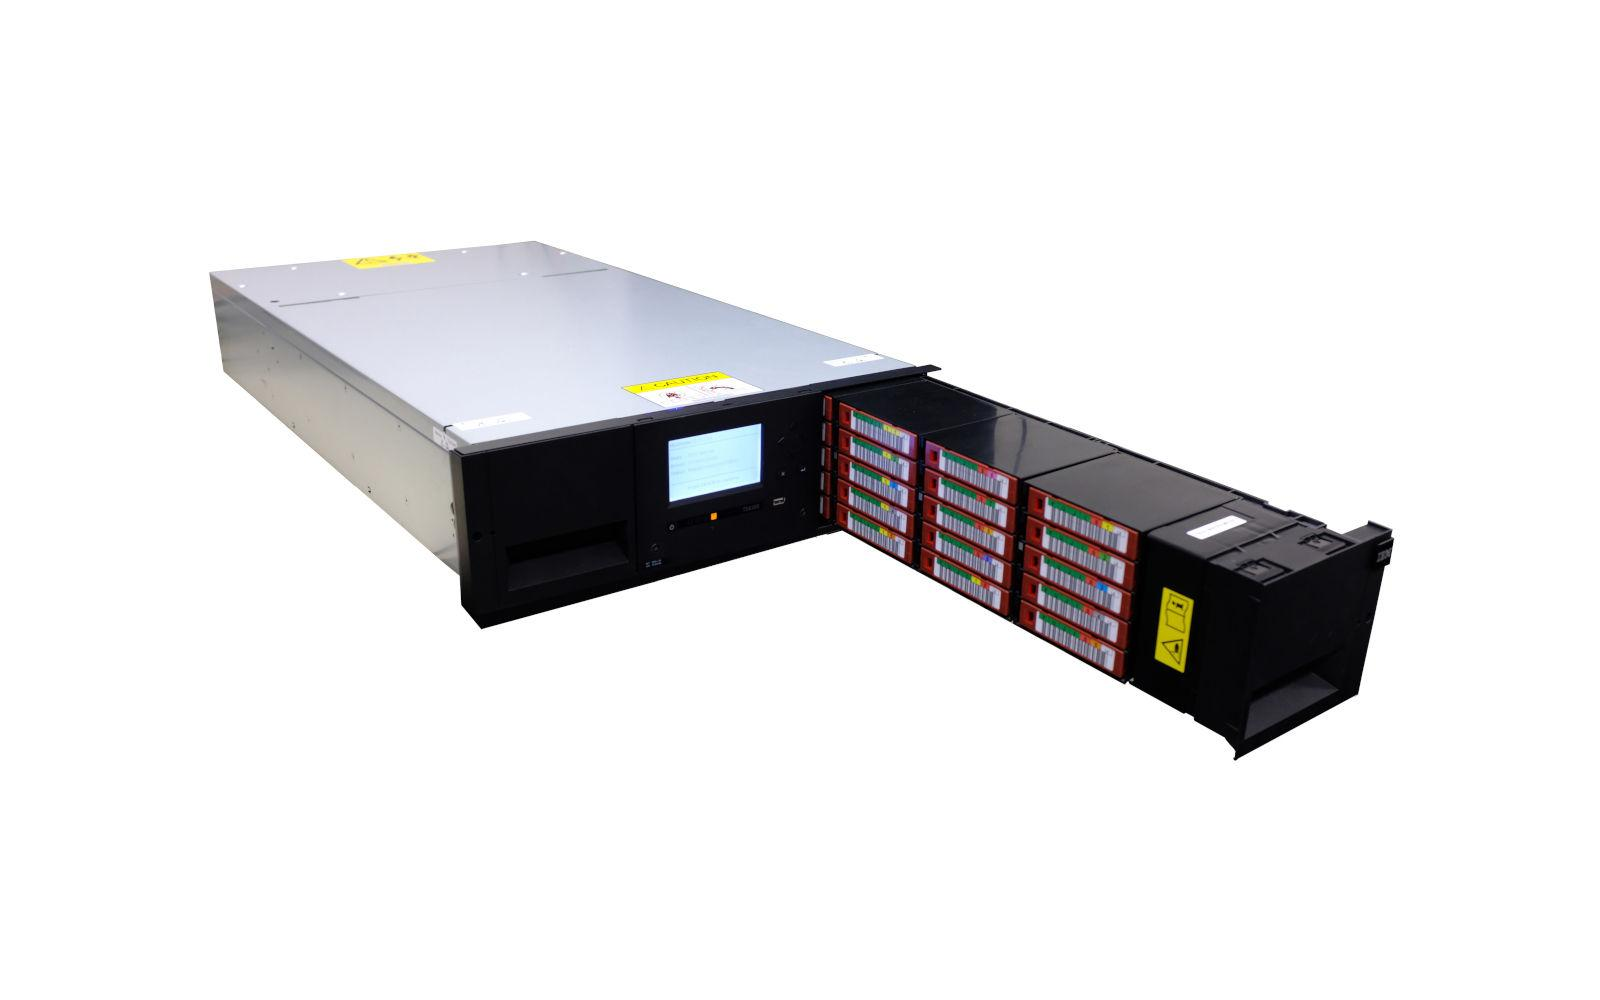
\includegraphics[scale=0.15]{cinta-magnetica.jpg}
        \caption{Lector de cintas magnéticas}
    \end{figure}

    \item \textbf{Discos Duros}

    El \textbf{disco duro} o \textbf{HD} (Hard Disk) es un dispositivo de almacenamiento de \textbf{acceso directo} que emplea un sistema de grabación magnética para almacenar los datos digitales.

    Esta compuestos por uno o más discos rígidos, de aluminio o material vitrocerámico, que se recubren de una fina capa de materia magnetizable, encerrados en un caja sellada, para evitar la entrada de impurezas que puedan perjudicar su funcionamiento. \textbf{Registran la información} mediante \textbf{variaciones en el campo magnético}, de forma que un punto puede estar magnetizado en un sentido u otro, representando un 1 ó un 0.

    Los \textbf{discos rígidos}, también llamados platos, están unidos por un eje a un motor que los hace girar simultáneamente a gran velocidad. En la actualidad, esta velocidad suele estar comprendida entre las 5.400 rpm y las 7.200 rpm.

    Entre los platos, se colocan unos \textbf{brazos metálicos} en cuyos extremos se sitúan los cabezales. Cada cabezal tiene dos cabezas para cada disco: una de lectura y otra de escritura, que son las que graban o leen la información usando pulsos magnéticos. Mientras estos platos giran, los brazos metálicos integrados en un mecanismo llamado \textbf{peine}, pueden desplazarse de forma perpendicular al eje de los platos. Combinando ambos movimientos, el cabezal de cada plato que va situando en el extremo del peine , puede llegar a cualquier punto de la superficie sin llegar a tocarla.

    Adicionalmente, los discos duros también disponen de una \textbf{parte electrónica} o de \textbf{control}, encarga de gestionar tanto el movimiento de los motores para posicionar los cabezales en el lugar adecuado, como la acción de los cabezales para que puedan escribir y leer, y por supuesto, para el control de la transferencia de información entre el propio disco duro y el computador.

    La \textbf{estructura lógica} que utilizan los discos duros para almacenar la información se les fija desde fábrica mediante un formateo de bajo nivel y es la siguiente:

    \begin{itemize}
        \item A cada disco se les aplica una estructura de \textbf{pistas}, \textbf{cilindros} y \textbf{sectores}, numerados de forma que el disco acaba dividido en un número de sectores físicos del mismo tamaño. Esta numeración permite accedes a cada sector de forma independiente al resto, convirtiendo a los discos duros en dispositivos de acceso directo.
        \item La \textbf{capacidad total} de almacenamiento de un disco se puede obtener multiplicando 521 bytes por el número de sectores, pistas y platos que tiene el disco.
        \item Una \textbf{pista} de un disco es cada una de las circunferencias concéntricas en las que se dividen sus caras. Las pistas se numeran desde la parte exterior empezando por 0. El número de pistas variará en función de la densidad de su material magnetizable y/o de las características particulares de los cabezales de lectura/escritura.
        \item Un \textbf{cilindro} es el conjunto de pistas ``en vertical'' sobre las que se posicionan las cabezas en un momento dado, un pista por cada cara del disco, que ocupan la misma posición. Así un disco tendrá tantos cilindros como pistas tenga cada una de sus caras.
        \item Ya que todos los cabezales se desplazan al unísono, es mas eficiente completar cilindros que caras.
        \item Las pistas, a su vez se dividen en sectores. Cada \textbf{sector} define la zona del disco duro en la que debe situarse el cabezal de lectura/escritura para leer o grabar la información. Además, el tamaño del sector determina la unidad mínima de información a la que pueden acceder los cabezales.
    \end{itemize}

    \begin{figure}[ht]
        \centering
        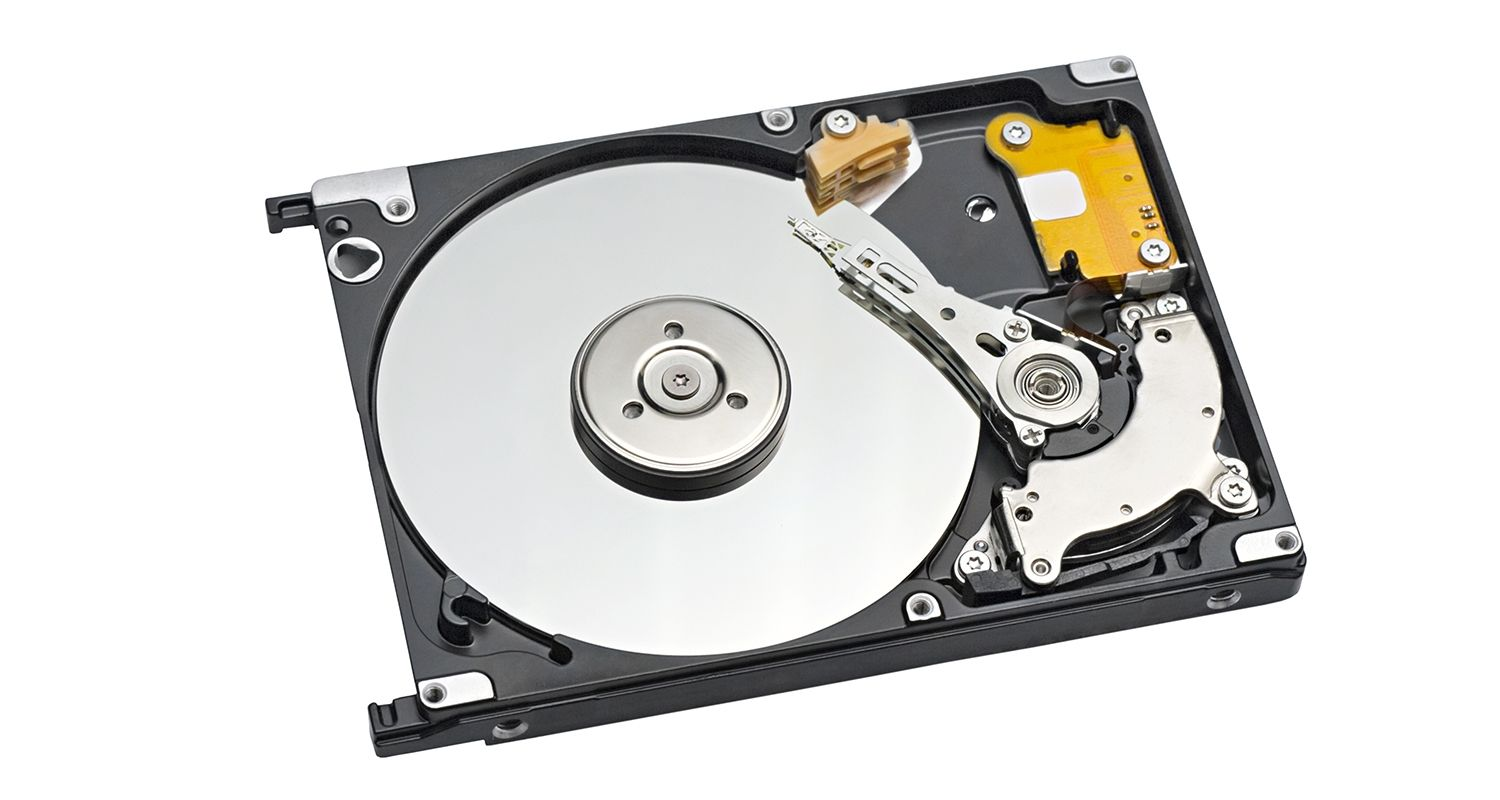
\includegraphics[scale=0.25]{disco-duro.jpg}
        \caption{Interior de un disco duro}
    \end{figure}

    Para la conexión de los discos duros al ordenador podemos utilizar diferentes interfaces, cada una con sus características propias, ya que usan diferentes tipos de cables y conectores, pero lo más importante es que cada tipo de interfaz utiliza un controlador diferente para gestionar la transmisión de información, como el modo o la velocidad.
    Las \textbf{interfaces} más usadas son estas:

    \begin{itemize}
        \item \textbf{ATA o PATA} (Parallel ATA): mas conocida como \textbf{IDE} (Integrated Device Electronics) y sus variaciones. Están quedando desfasados debido al uso cada vez mas extendido de las interfaces SATA. La \textbf{velocidad} de su mejor versión llegaba a soportar \textbf{166 MB/s}.

        \item \textbf{SATA} (Serial ATA): utiliza un bus de serie para la transmisión de datos, siendo mas rápido y eficiente que el bus en paralelo de IDE. Existen tres versiones, \textbf{SATA 1, 2 y 3} con velocidades de transferencia de hasta \textbf{150}, \textbf{300} y \textbf{600 MB/s} respectivamente.

        \item \textbf{SCSI}: sin interfaces preparadas para discos de gran de capacidad de almacenamiento y gran velocidad de rotación que se utilizan en \textbf{servidores} a nivel profesional. Existen tres versiones, \textbf{SCSI Estándar} (Standard SCSI), \textbf{SCSI Rápido} (Fast SCSI) y \textbf{SCSI Ancho-Rápido} (Fast-Wide SCSI), con velocidades de \textbf{5}, \textbf{10} y \textbf{20 MB/s} respectivamente. También podemos encontrar la versión \textbf{SAS} (Serial Attached SCSI), una versión nueva y más rápida que las versiones en paralelo.
    \end{itemize}

    \item \textbf{Lectores de CD-ROM}

    Son dispositivos electrónicos que usan \textbf{tecnología óptica}, el láser, para leer la información grabada en discos o CDs, que con intercambiables. Usualmente disponen de una bandeja que sale y entra del dispositivo para alojar el disco que se va a utilizar, aunque hay modelos que solo disponen de un abertura por la que introducir y expulsar los discos.

    \begin{figure}[ht]
        \centering
        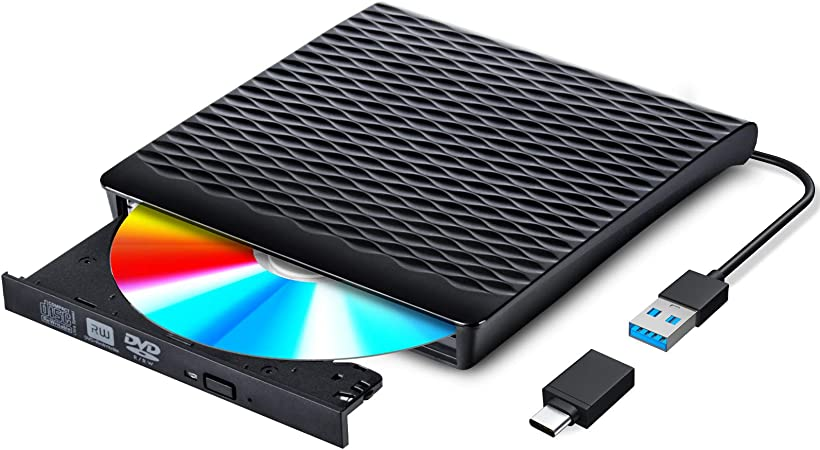
\includegraphics[scale=0.35]{grabadora-cd.jpg}
        \caption{Grabadora de CD/DVD	 externa}
    \end{figure}

    Los \textbf{discos} o \textbf{CDs}, son discos rígidos de 8 a 12 cm de diámetro, con un orificio central de 15 mm de diámetro y un grosor de 1,2 mm, que pueden almacenar entre 214 MB y 700 MB de información respectivamente. Están formados por varias capas de policarbonato que recubren un finísima capa de aluminio reflectante.

    La información esta grabada en una \textbf{única pista} en \textbf{espiral} que se inicia en el centro de y se dirige hacia el exterior. Siguiendo esa pista y bajo la capa reflectante esta grabada la información en binario por medio de microsurcos que representan los 1s y los 0s.

    Para leer el CD se utiliza un \textbf{emisor de luz} que envía un fino \textbf{haz láser} hacia la superficie del disco con una determinada \textbf{amplitud de onda}. El reflejo es capturado por un \textbf{fotoreceptor} que cuantifica la cantidad de luz reflejada y determina si dicho reflejo viene de una zona lisa, cuando mantiene la misma amplitud, o de una zona con surco, cuando tiene la mitad de amplitud de la onda original.

    En contra de lo que se suele pensar, las zonas de distinta profundidad, \textbf{llanos y surcos}, no representan los ceros y los unos, sino que en realidad los valores binarios son determinados cuando se detecta el salto entre una zona y otra. Un salto se interpreta como un 1 binario, mientras que la longitud de un surco se interpreta como una sucesión de 0s binarios.

    El \textbf{lector de disco} tiene un motor que hace rotar el disco, y otro que mueve el cabezal radialmente. Con la combinación de ambos movimientos, el láser tiene acceso a todo el disco. La velocidad de giro es controlada por un microprocesador que actúa en función de la posición del cabezal de lectura, para permitir un acceso aleatorio a los datos. Así, cuanto más cerca del borde del disco esté el cabeza de lectura, mas lento girará éste.

    Hay unidades \textbf{grabadoras de CD-ROM} que permiten grabar ciertos discos. En realidad, son unidades lectoras a las que se les incorpora un nuevo láser con una frecuencia diferente, que permite modificar la superficie del disco en forma de llanos y surcos para almacenar la información en binario. Los \textbf{CDs grabables} deben tener una capa de material fotosensible que puede ser modificada por una determinada frecuencia de luz para poder ser grabados. Normalmente no se puede grabar más que una vez en un mismo disco, aunque los \textbf{CD-RW}, regrabables, si lo permiten, ya que la capa sobre la que se graba la información es de un compuesto químico que al enfriarse cristaliza de forma rápida, pero que al calentarse de nuevo recupera la estructura original.


    \item \textbf{Lectores de DVD}

    El \textbf{disco versátil digital} (Digital Versatil Disk) tiene una capacidad de almacenamiento y velocidades de transferencia muy superiores al los CDs, pudiendo llegar a albergar \textbf{hasta 17 GB de información} en total. Debido a esto, para que se pueda leer un DVD el láser debe tener una longitud de onda más pequeña.

    El aspecto de un DVD es similar al de un CD, pero puede tener una o\textbf{dos caras para la grabación de información}, dependiendo del número de capas reflectantes tenga, cada una de un grosor de 0.6 mm. Además de doblar la superficie de grabación por tener dos caras, los surcos se graban con un tamaño mucho menor, permitiendo así que la pista de datos se estreche, y por tanto, sea mucho más larga. Todo esto implica que pueda almacenar hasta 7 veces más información que un CD normal, por lo que puede almacenar hasta 9,4 GB de información.

    Otro formato de DVD permite tener 2 pistas de datos concéntricas superpuestas en un misma cara. Cada pista tiene indices de reflexión diferentes y transparencia diferentes, lo que permite que la lectora pueda acceder a ambas solo con cambiar el enfoque y la intensidad del láser, permitiendo así tener dos pistas de 8.5 GB cada una, lo que nos da un total de 17 GB de información.

    Tanto los \textbf{CDs} como los \textbf{DVDs}, pueden conectarse al ordenador mediante las mismas interfaces que los discos duros, esto es: \textbf{IDE}, \textbf{SATA} y \textbf{SCSI}.

    \item \textbf{Blu-Ray}

    El \textbf{Blu-ray disc} o \textbf{BD} fue desarrollado para la ejecución de vídeo de altísima calidad, aunque también puede ser utilizado para el almacenamiento de datos. Es un nuevo formato de disco óptico que manteniendo las medidas del CD y el DVD, puede llegar a almacenar \textbf{hasta 100 GB} de información.

    Cada capa de un disco de Blu-ray puede almacenar hasta 25 GB, y existen discos de hasta 4 capas. La mayor densidad de información se consigue gracias al uso del \textbf{láser azul}, que le da nombre al formato, que con su \textbf{longitud de onda de 405 nm}, frente a los \textbf{650 nm del láser rojo} del DVD, le permite almacenar más información por unidad de superficie.

    Existen varios formatos de Blu-ray: \textbf{BD-R}, regrabable, \textbf{BD-RE}, formato reescribible y \textbf{BD-ROM}.

    A diferencia del CD y DVD, solo puede conectarse al ordenador mediante una interfaz \textbf{SATA}.

    \item \textbf{Tarjetas de Memoria Flash}

    La flash, es un tipo de \textbf{memoria no volátil} que viene encapsulada en pequeñas tarjetas de plástico cuya capacidad y velocidad dependerá de los chips de memoria que lleve en su interior.

    En un principio fueron inventadas para usarse como soporte de memoria exterior para dispositivos como teléfonos móviles y PDAs, reproductores musicales, cámaras de fotos, etc.., pero como el tiempo se han extendido su uso también como dispositivo de almacenamiento de uso general.

    Existen \textbf{multitud de formatos}, debido a que los fabricantes, en función de sus intereses, crearon sus propios diseños creando sus formas, tamaños, número de conectores, capacidad, etc.., con el fin de utilizarlos en los aparatos para los que habían sido diseñados. Incluso existen adaptadores para poder usar una misma tarjeta en dispositivos con diferente formato, pero al tratarse de dispositivos de memoria digital, los \textbf{ordenadores} han tardado poco en \textbf{incorporar los lectores} adecuados para la lectura de este tipo de dispositivos.

    \begin{figure}[ht]
        \centering
        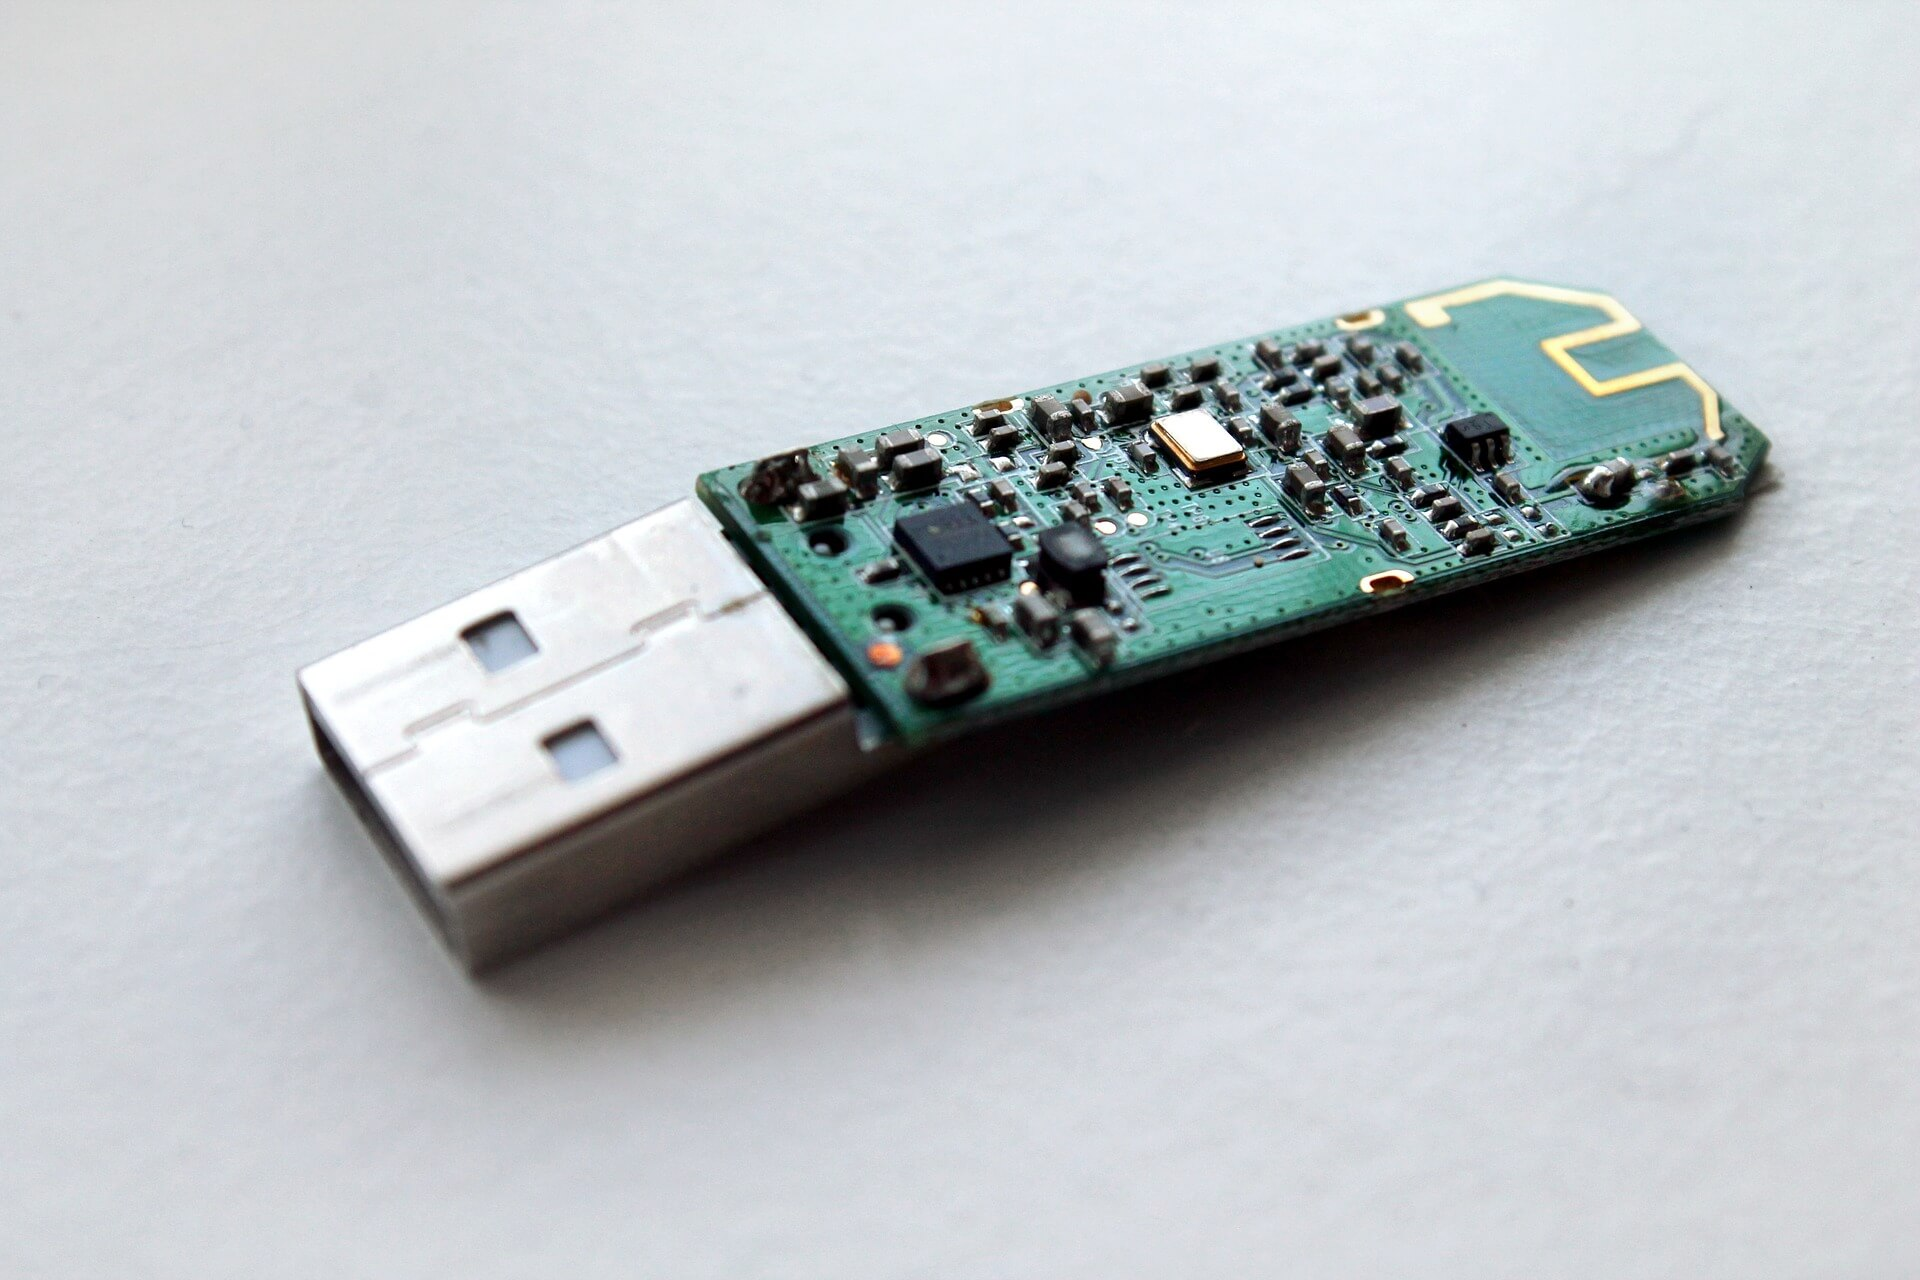
\includegraphics[scale=0.15]{memoria-flash.jpg}
        \caption{Memoria flash sin la carcasa}
    \end{figure}

    Dentro de los diferentes formatos de memoria flash que existen, los más comunes son:

    \begin{itemize}
        \item CompactFlash (CF)
        \item SmartMedia Card (SMC)
        \item Memory Stick y Memory Stick PRO
        \item Secure Digital (SD)
        \item Secure Digital High Capacity (SDHC)
        \item Pendrives y Memorias USB.
    \end{itemize}
\end{itemize}

\section{Montaje de un Ordenador Personal}
En esta sección vamos a realizar el ensamblado de un ordenador personal de sobremesa. Para ello deberemos seguir unos pasos que se detallarán en la segunda sección de este apartado, pero primero tendremos que hacer un inventario y comprobar que disponemos de las herramientas necesarias, así como tener claro algunas precauciones, lo que veremos en el siguiente punto.

\subsection{Preparación}
Antes de ponernos a montar el ordenador, deberemos de prepararnos para el proceso de ensamblado, lo que deberemos hacer siguiendo los siguiente pasos:

\begin{enumerate}
    \item \textbf{Inventario}

    En primer lugar, vamos a hacer un repaso del hardware que tenemos para montar el ordenador, en nuestro caso, las piezas que vamos a usar son las siguientes:

    \begin{itemize}
        \item \textbf{Caja de tipo semitorre} que contiene:
        \begin{itemize}
            \item La fuente de alimentación
            \item Los tornillos necesarios para fijar los componentes.
            \item Los cables del panel frontal para la conexión de los LED indicadores y los pulsadores de reinicio y apagado.
            \item Los cables del panel frontal para la conexión de dispositivos USB y de sonido
            \item Un pequeño altavoz.
            \item Una placa que se añade por si es necesario tapar el hueco de la caja que ya viene hecho de fábrica
        \end{itemize}

        \item \textbf{Placa base}, modelo G41T-R3 de la marca ELITEGROUP, con vídeo, sonido y red integrados. Es apropiada para el procesador que vamos a utilizar. Además, en la misma caja vienen embalados:

        \begin{itemize}
            \item El manual de placa base y el CD con sus drivers.
            \item La placa base, empaquetada en una bolsa de plástico antiéstatico.
            \item Dos cables de datos SATA, para las unidades de almacenamiento internas.
            \item Una plaquita de metal adaptada a los huecos de los conectores externos de la placa.
        \end{itemize}

    \item \textbf{Disco duro} de tipo SATA con 250 GB de capacidad.
    \item La unidad óptica es un \textbf{grabador/lector de DVD} con conexión SATA.
    \item \textbf{Lector de tarjetas} de memoria flash.
    \item \textbf{Memoria RAM}, un solo modulo DIMM de 2 GB de capacidad a 1066 MHz de tipo DDR3.
    \item \textbf{El procesador} es un Pentium de la marca Intel modelo E6700 LGA775, totalmente compatible con el zócalo de la placa base que hemos adquirido. Empaquetado en su misma caja viene el conjunto disipador ventilador que vamos a utilizar para su refrigeración.
    \item \textbf{Tarjeta de vídeo} para zócalo PCI Express con ventilación pasiva (con disipador pero sin ventilador) y con conexiones externas de tipo SVGA, DVI y HDMI.
    \item \textbf{Tarjeta de red inalámbrica} de tipo PCI, para disponer de conexión Wi-Fi
    \item \textbf{Jeringuilla de pasta térmica} para poner entre el procesador y el disipador.
    \end{itemize}

    \item \textbf{Herramientas Necesarias}

    Una vez que hemos hecho un inventario del hardware que vamos a emplear para montar nuestro PC, vamos a ver si disponemos de las herramientas que necesitaremos en el proceso de ensamblado. Estas son:

    \begin{itemize}
        \item Destornillador de estrella (o Philips) para abrir y cerrar la caja y para fijar los componentes.
        \item Un destornillador plano puede ser útil para retirar alguna placa metálica o plástica haciendo palanca.
        \item Alicates pequeños con punta delgada para apretar los tornillos separadores.
        \item Pinzas alargadas y finas para poder recuperar tornillos de zonas poco accesibles en caso de ser necesario.
        \item Pulsera antiestática para evitar posibles descargas dañinas sobre los componentes.
    \end{itemize}

    \item \textbf{Precauciones y Advertencias de Seguridad}

    Antes de lanzarnos a montar el ordenador, cabe tener en cuenta unas cuantas consideraciones de seguridad para no llevarnos algún susto. Las principales a tener en cuenta son:

    \begin{itemize}
        \item Las conexiones y desconexiones que se realicen sobre la placa base deben realizarse con el ordenador apagado y desconectado de la toma de corriente eléctrica. De esta forma se evitan cortocircuitos e incluso incendios. Por si acaso debe tener a mano un extintor adecuado para elementos electrónicos.

        \item Para trabajar cómodamente se necesita disponer de una amplia superficie de trabajo, suficientemente iluminada, sobre la que colocar tanto los componentes como las herramientas necesarias. Procure alejar de esta zona cualquier clase de líquido y cualquier cosa que produzca electricidad estática como alfombras, moquetas, mantas, etc...

        \item Debe tenerse especial cuidado en auto descargarse de nuestra posible electricidad estática a la hora de manipular componentes para evitar que esta les produzca algún tipo de daño, de no hacerlo, elementos como las memorias se podrían dañar y quedar inutilizadas. Para ello se debe tocar algún elemento metálico como la propia caja del ordenador o utilizar una pulsera antiestática.

        \item Es necesario contar con un juego de herramientas adecuadas, entre las que se deben incluir una pulsera antielectricidad estática, destornilladores planos y de estrella que estén imantados, pequeños alicates, pinzas, etc...

        \item Todos y cada uno de los conectores que se utilizan en la placa base y por extensión en el ordenador tienen un diseño único en su forma y en la disposición de sus contactos que les impide ser insertados erróneamente en donde no les corresponda.

        \item Para trabajar con seguridad es conveniente no llevar puestos abalorios como colgantes, pulseras, relojes, anillos, etc. que puedan rozar o engancharse en algún elemento, esto es también aplicable a la ropa "suelta" tipo corbata, fular, mangas anchas, etc...

        \item Algunos componentes, como placas base o tarjetas de expansión, tienen en su parte posterior los extremos de los componentes que sobresalen de las soldaduras como pequeños pinchos que pueden clavarse en la piel. Por lo que se aconseja que estas placas se manipulen cogiéndolas por los cantos.

        \item Hay que poner especial cuidado para evitar que puedan producirse heridas de forma involuntaria por ejemplo al rozarse con algún componente o al cortarse con los cantos afilados de alguna chapa, o al pellizcarse mientras se inserta o extrae algún elemento o incluso si nos cae encima algún elemento pesado mientras se manipula. También hay que evitar tocar los elementos que puedan estar calientes como el procesador, o que trabajen con alto voltaje como la fuente de alimentación o el monitor.
    \end{itemize}
\end{enumerate}

Una vez que ya seguido estos pasos y recordado algunas consideraciones de seguridad estamos listos para empezar con el proceso de montaje. Para ello, en la siguiente sección, se ira explicando paso por paso que debemos hacer.

\subsection{Proceso de Montaje}






% Apéndice
\appendix

% Change appendix display options
\titleformat{\chapter}{\bfseries\Huge}{\thechapter.}{1ex}{}

\chapter{Anexos Tema 1}

\section{Clasificación de Ordenadores}
En este anexo vamos a realizar una clasificación de los ordenadores según su potencia de computación y tamaño, de mayor a menor, pudiendo diferenciar 5 tipos de computador:

\begin{enumerate}
    \item \textbf{Supercomputador o Superordenador}

    Un superordenador es un ordenador extraordinariamente rápido con capacidades de proceso, cálculo, almacenamiento, etc.., muy superiores tecnológicamente comprado con el resto de ordenadores construidos en la misma época.

    Físicamente son de gran tamaño y deben ser instalados en ambientes controlados para poder disipar todo el calor que generan sus componentes, lo que no impide que puedan soportar la conexión de miles de usuarios simultáneamente o realizar cálculo extremadamente complejos.

    Suelen incluir varios procesadores de gran potencia que trabajan conjuntamente, en paralelo, destinados a una tarea específica. En número de procesadores, dependiente del modelo, varía entre los 16 procesadores hasta 512. Por supuesto, también cuentan con una generosa cantidad de memoria y con gran capacidad de almacenamiento. Esto les permite procesar ingentes cantidades de información en poco tiempo, pudiendo llegar a procesar miles de millones de operaciones por segundo.

    Debido a su gran potencia, suelen ser utilizados para realizar simulaciones de procesos muy complejos con gran cantidad de datos, como por ejemplo, el análisis de genoma humano,la simulación de explosiones nucleares, predicciones meteorológicas o astronómicas, etc.., pero también son empleados para diseñar y simular máquinas complejas como automóviles o aviones, y para controlar el funcionamiento de las naves espaciales y satélites, entre otras cosas.

    \begin{figure}[ht]
        \centering
        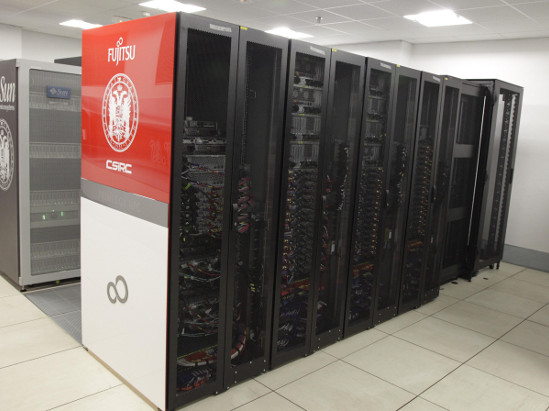
\includegraphics[scale=0.36]{ugr-grid.jpg}
        \caption{Supercomputador UGRgrid de la Universidad de Granada}
    \end{figure}

    \item \textbf{Mainframes}

    Los mainframes son grandes ordenadores, de uso general, que disponen de varios procesadores que pueden trabajar de forma independiente entre sí, pudiendo así realizar varias tareas simultáneamente. Están preparados para realizar varios millones de operaciones por segundo. Su gran capacidad de proceso le permiten, por un lado, controlar al mismo tiempo a cientos incluso miles de usuarios y por otro lado controlar el manejo de puertos de salida y de entrada, dando soporte a cientos de dispositivos de entrada y salida, gracias a lo cual pueden contar con muchas unidades de disco que les permiten almacenar grandes cantidades de información.

    Físicamente hoy en día un mainframe tiene la apariencia de una fila de archivadores,similares a los de una biblioteca, que se suelen instalar en una habitación con un control de temperatura y con doble suelo, bajo el que se alojan la gran cantidad de cables necesarios para la conexión de periféricos.

    En comparación con un superodenador, un mainframe es mucho más barato y puede ejecutar simultáneamente mayor numero de programas, pero los superordenadores pueden ejecutar un solo programa mucho mas rápido.

    Son utilizados en las empresas de gran tamaño, con muchas sucursales como bancos, compañías de transporte, etc...

    \begin{figure}[ht]
        \centering
        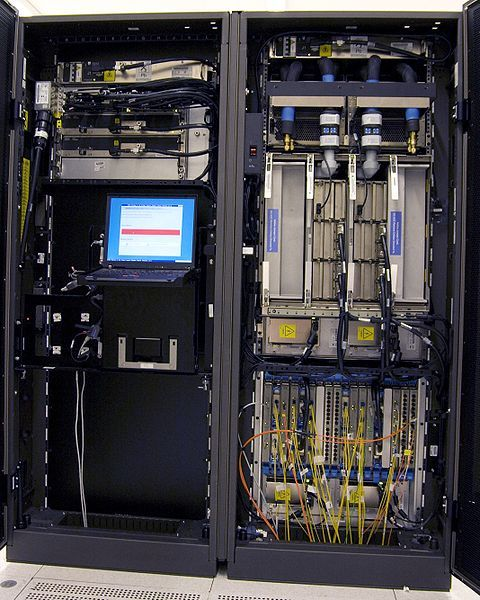
\includegraphics[scale=0.30]{mainframe.jpg}
        \caption{Mainframe}
    \end{figure}

    \item \textbf{Minicomputadora o Miniordenador}
    Son una versión reducida de los mainframes, con menos prestaciones de velocidad, menos memoria, menor capacidad de almacenamiento y menos número de terminales. Están orientadas a tareas específicas. Fueron ideadas para dar servicio a empresas e instituciones, de menor tamaño, que no necesitan toda la capacidad de procesamiento ni los periféricos que aporta un mainframe.

    Un minicomputador es, por tanto, un sistema multiproceso y multiusuario que ofrece servicios específicos, que cuenta con capacidad de soportar hasta 200 usuarios conectados simultáneamente y que soporta un número limitado de dispositivos. Son de relativo pequeño tamaño y costo comparados con un mainframe.

    Se suelen utilizar para el almacenamiento de grandes bases de datos, para el control automático en la industria y para aplicaciones multiusuario.

    \vspace{5ex}

    \item \textbf{Workstation o Estación de Trabajo}

    Una estación de trabajo es un ordenador de gran potencia para ser usado por un solo usuario. Es parecido a un ordenador personal pero con mejores componentes, que le proporciona mayor potencia y calidad, y que normalmente se conecta a un ordenador más grande mediante una conexión de red, permitiendo a los usuarios compartir ficheros, aplicaciones y hardware, como impresoras.

    \begin{figure}[ht]
        \centering
        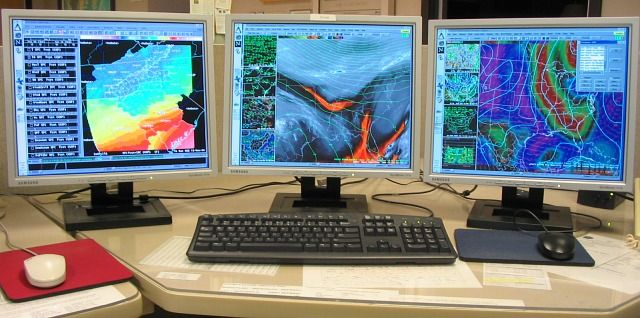
\includegraphics[scale=0.40]{workstation.jpg}
        \caption{Estación de trabajo con 3 monitores}
    \end{figure}

    Internamente las estaciones de trabajo suelen estar basadas en otro diseño de CPU llamado RISC (Reduced Instruction Set Computer), con el que las instrucciones de procesan de forma más rápida. Suelen emplearse para aplicaciones de ingeniería, CAD (Computer Aided Design), diseño de publicidad, programación de software, etc...

    \item \textbf{Ordenador Personal o PC}

    Conocido como PC (Personal Computer), es un ordenador de propósito general general, de pequeño tamaño, con al menos un microprocesador, que suele disponer de ratón y teclado para introducir los datos y de un monitor para mostrar la información, además de algún dispositivo de almacenamiento en el que instalar el sistema operativo y guardar datos y programas. También admite la conexión de otros periféricos con múltiples y variadas funciones.

    Son los ordenadores más accesibles para cualquier tipo de usuario, en cuanto a coste y facilidad de uso. En sus inicios solo podían trabajar en modo monousuario, pero con los avances tecnológicos ahora pueden ser usados en modo multiusuario e incluso como servidores de una red de ordenadores.

        \begin{figure}[ht]
        \centering
        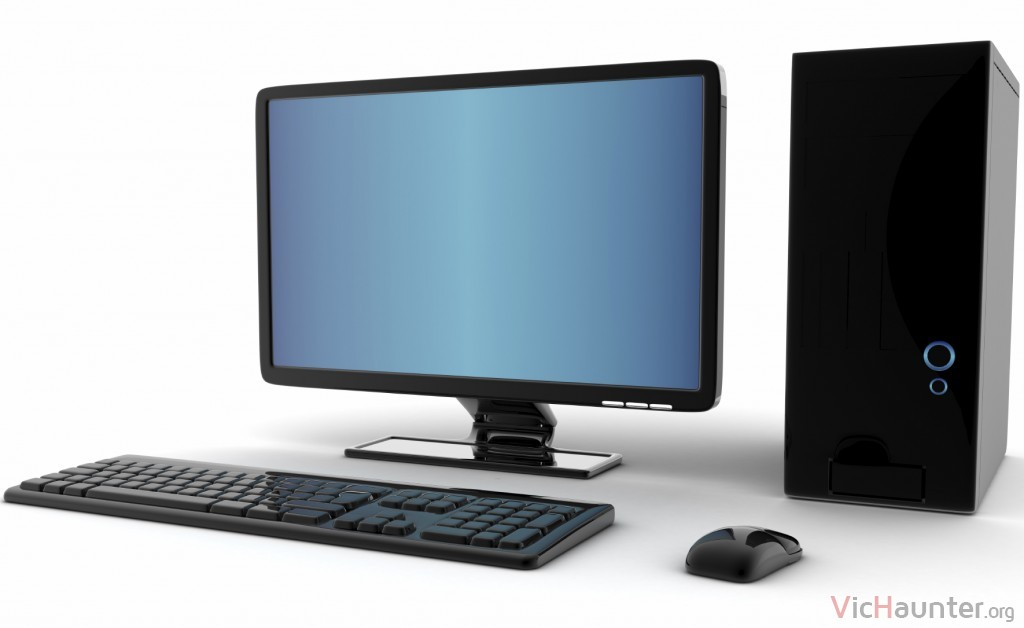
\includegraphics[scale=0.25]{pc.jpg}
        \caption{Ordenador Personal}
    \end{figure}

    Los PCs tuvieron su origen gracias a la creación de microprocesadores por parte de Intel, y a que IBM los incorporó en unos pequeños ordenadores que con el tiempo se estandarizaron, facilitando que otras compañías pudieran también fabricarlos y comercializarlos a precios asequibles para el gran público.
\end{enumerate}

\section{Tipos de Ordenadores Personales}
En la actualidad hay un gran variedad de ordenadores personales, con diferentes tamaños	y prestaciones, ya que este tipo de computador se ha diversificado mucho en los últimos 20 años. Los principales tipos de ordenadores que nos podemos encontrar hoy en día son los siguientes:

\begin{itemize}
    \item \textbf{Ordenador de Escritorio}: son uno de los tipos de ordenador personal más extendidos, salvando a los smartphones. Están diseñados y fabricados para instalarse en una ubicación estática, como un escritorio o una mesa, a diferencia de los portátiles. Son computadoras de uso doméstico que suelen estar dedicadas al entretenimiento y las tareas domesticas. Dentro de los PC, suelen ser los que tienen mas potencia y ofrecen más prestaciones.

    \begin{figure}[ht]
        \centering
        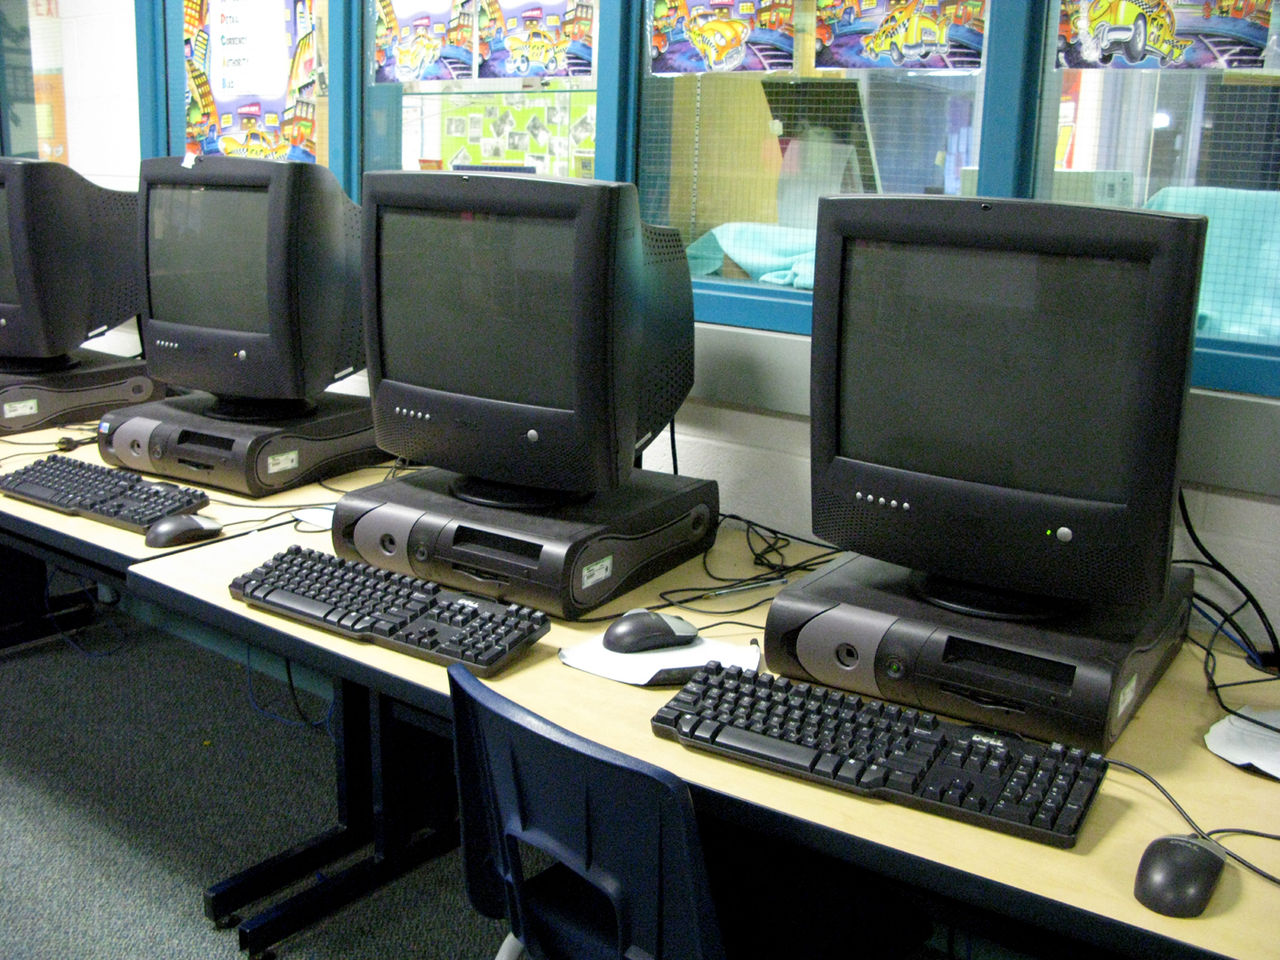
\includegraphics[scale=0.35]{ordenadores-escritorio.jpg}
        \caption{Sala con varios ordenadores de escritorio}
    \end{figure}

    \item \textbf{Ordenador Portátil o Laptop}: Es un ordenador personal que puede transportarse con facilidad por ser ligero de peso y de reducido tamaño.Están equipados con una batería que les permiten sin tener que estar conectados a la red eléctrica.

    \begin{figure}[ht]
        \centering
        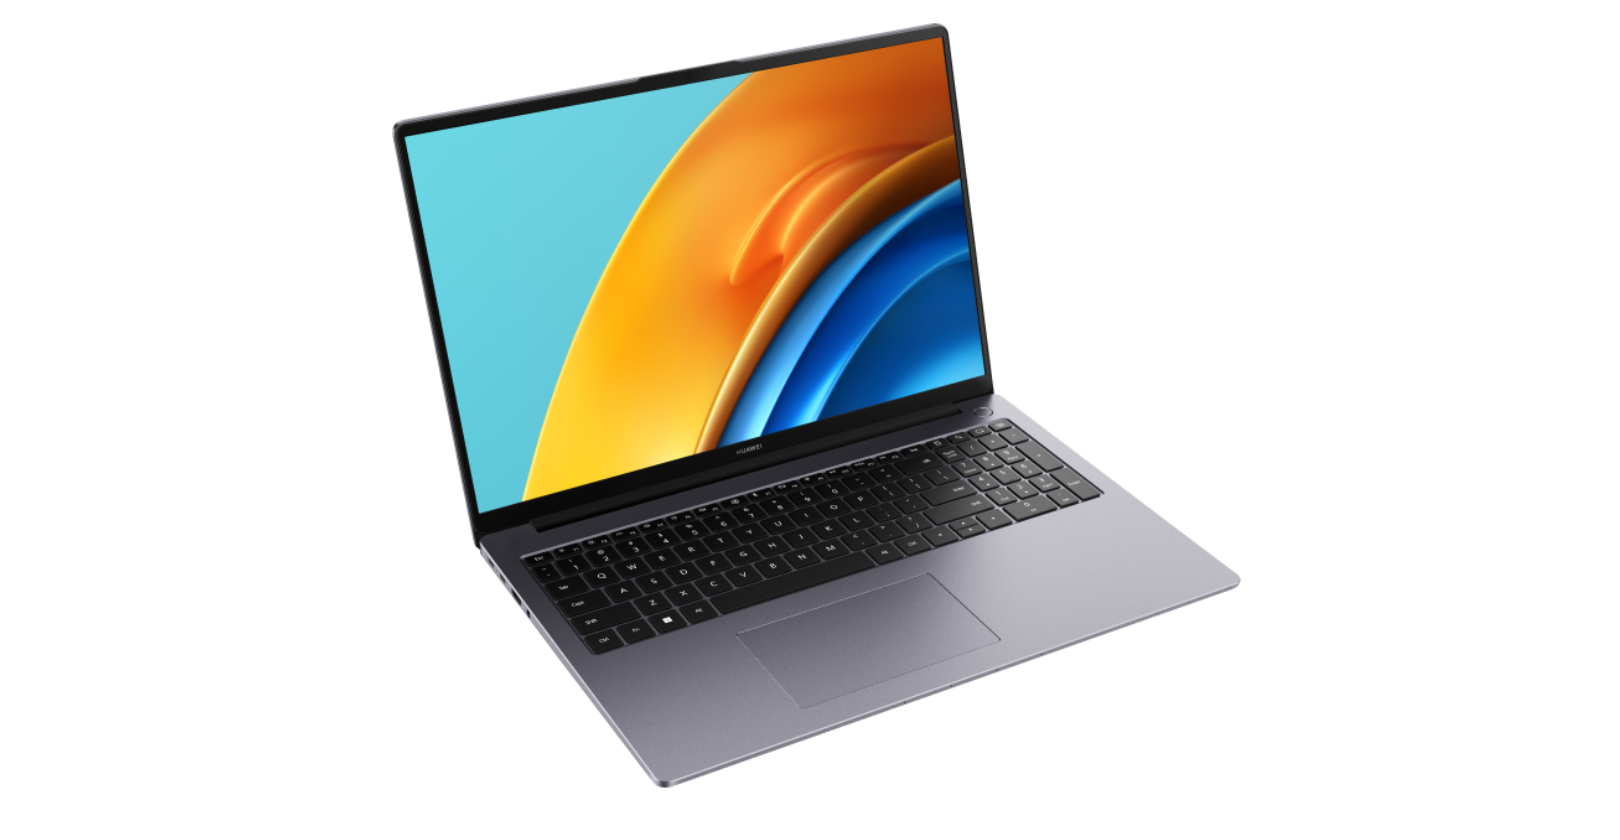
\includegraphics[scale=0.25]{ordenador-portatil.png}
        \caption{Ordenador Portátil}
    \end{figure}

    \item \textbf{Notebook}: es un ordenador portátil más pequeño que los laptop y que por norma general tiene menos potencia. Son más ligeros y suelen usarse para tareas que requieren poca potencia de procesado como navegar por internet.

    \item \textbf{TabletPC}: se trata de un ordenador pizarra sin teclado físico, que dispone de una pantalla táctil con la que se interactúa utilizando los dedos o algún tipo de apuntador. Hay portátiles que disponen de teclado y ratón y permiten girar la pantalla para usarlos a modo de TabletPC.

    \begin{figure}[ht]
        \centering
        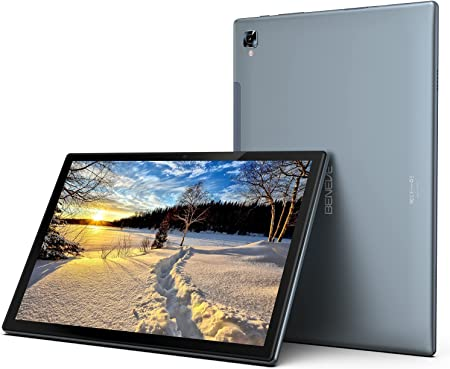
\includegraphics[scale=0.35]{tablet.jpg}
        \caption{Tablet PC}
    \end{figure}

    \item \textbf{Portátil Convertible}: son portátiles que disponen de un teclado físico y permiten rotar la pantalla sobre una bisagra o deslizar el teclado debajo de la pantalla, colocándose como si de una pizarra se tratara y permitiendo su uso como una TabletPC.

    \begin{figure}[ht]
        \centering
        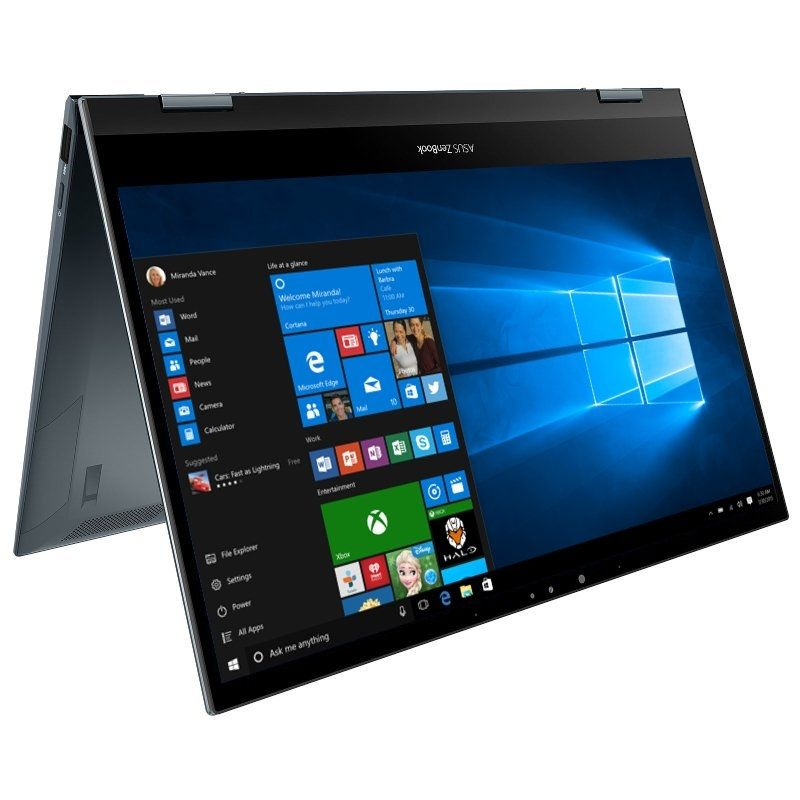
\includegraphics[scale=0.18]{portatil-convertible.jpg}
        \caption{Ordenador portátil convertible}
    \end{figure}

    \item \textbf{Pocket o PDA}: es un ordenador pequeño que cabe en la palma de una mano y tiene muchas de las prestaciones de los ordenadores de escritorio, pero no todas.

    \begin{figure}[ht]
        \centering
        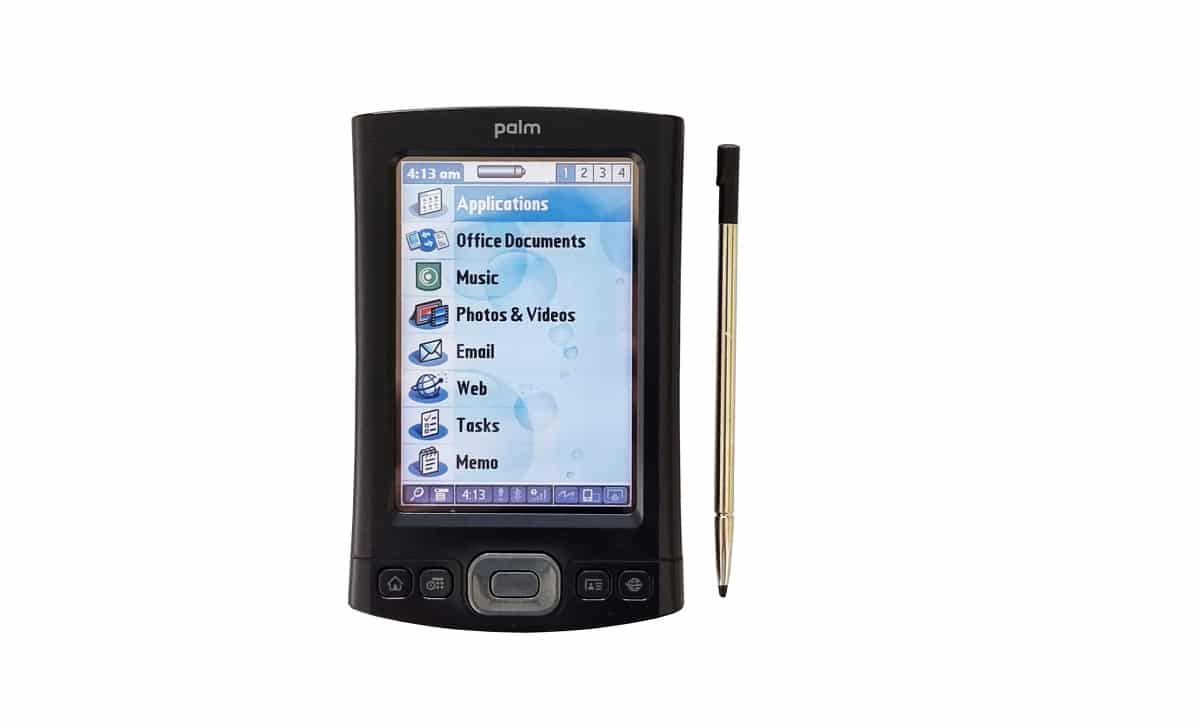
\includegraphics[scale=0.14]{pda.jpg}
        \caption{PDA con su lápiz}
    \end{figure}

    \item \textbf{Smartphone}: es un teléfono móvil que incorpora características de un ordenador personal. Pueden tener un mini teclado, una pantalla táctil, un lápiz óptico, etc... Incluyen un acceso a Internet, servicios de correo electrónico, cámara integrada, navegador web, procesador de textos, etc... Permiten la instalación de una gran variedad de aplicaciones con las que aumentar sus funcionalidades. Actualmente, es el ordenador personal más extendido en el mundo.

    \begin{figure}[ht]
        \centering
        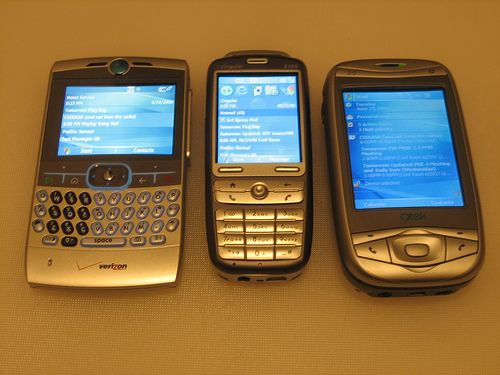
\includegraphics[scale=0.35]{smartphones.jpg}
        \caption{Diferentes tipos de Smarthphones}
    \end{figure}

    \item \textbf{Mini PC}: es un ordenador en una barra USB. En sus pequeñas dimensiones integra un puerto HDMI, USB y microUSB (a los que se les puede conectar un disco duro externo), microSD y además disponen de conectividad interna Wi-Fi. El precio, al no incluir pantalla, suele ser más asequible que las TabletPC.

    \begin{figure}[ht]
        \centering
        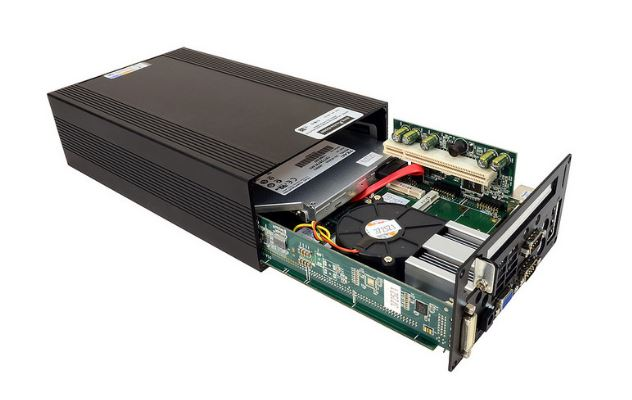
\includegraphics[scale=0.38]{minipc.jpg}
        \caption{MiniPC abierto}
    \end{figure}
\end{itemize}

Todos estos ordenadores personales pueden funcionar con diferentes sistemas operativos.  Estos se dividen en dos tipos:

\begin{itemize}
    \item Sistemas operativos basados en escritorio.
    \item Sistemas operativos pos-PC (similares a los SO de los smarthphones)
\end{itemize}

En la actualidad, los SO más populares en cada tipo son: Microsoft Windows y sistemas GNU/Linux para los basados en escritorio, e iOS de Apple y Android de Google para los pos-PC. También muchos fabricantes están probando productos como Chrome OS de Google, y otros, principalmente asiáticos, están incorporando doble sistema operativo, permitiendo operar con diferentes sistemas operativos como Android y Windows según las necesidades del usuario.

\section{Principales Conectores de la Placa Base}
En este anexo vamos a ver de forma detallada cuales son todos los conectores que incluye una placa base y cual es su utilidad, para que podamos identificarlos cuando vayamos a montar un ordenador o simplemente cuando tengamos una placa base delante.

\begin{itemize}
    \item \textbf{Zócalo del Microprocesador}
    Es donde va insertado la CPU del ordenador. Según la forma de inserción podemos encontrarnos de varios tipos:

    \begin{itemize}
        \item \textbf{ZIF} (Zero Insertion Force): también llamados comúnmente \textbf{PGA} (Pin Grid Array), aunque este último nombre hace referencia a la disposición de los pines en el procesador. Tiene un mecanismo que permite introducir las pastillas del procesador sin hacer presión para evitar que pueda estropearse. Una palanca que gira hace que se ajusten los contactos. Para su retirada, el movimiento contrario de la palanca hace que el procesador quede suelto y sea muy fácil retirarlo.

        \begin{figure}[ht]
            \centering
            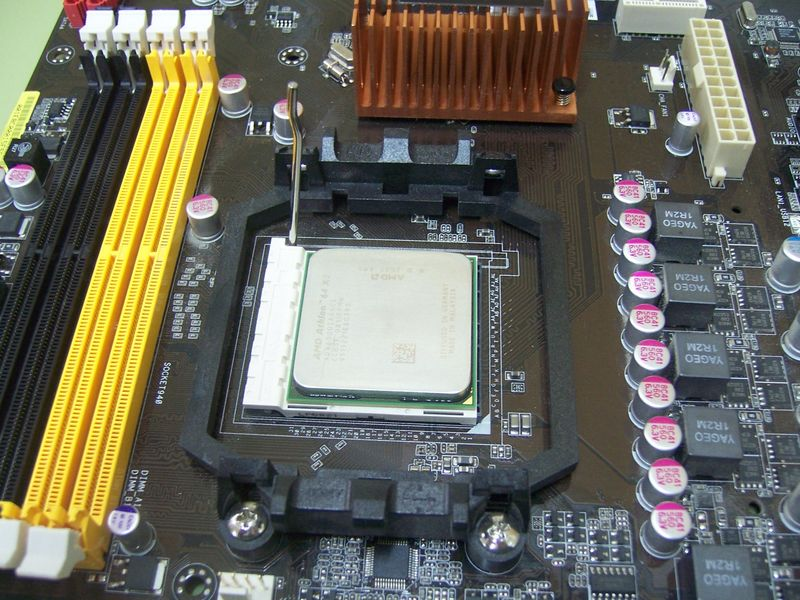
\includegraphics[scale=0.28]{mb-zif.jpg}
            \caption{Zócalo de tipo ZIF}
        \end{figure}

        \item \textbf{LGA} (Land Grid Array): en este caso los pines se encuentran en el propio zócalo mientas que los contactos del procesador son planos. También hay una palanca que ajusta el procesador al zócalo con ayuda de una especie de marco metálico que lo rodea manteniéndolo inmovilizado.

        \begin{figure}[ht]
            \centering
            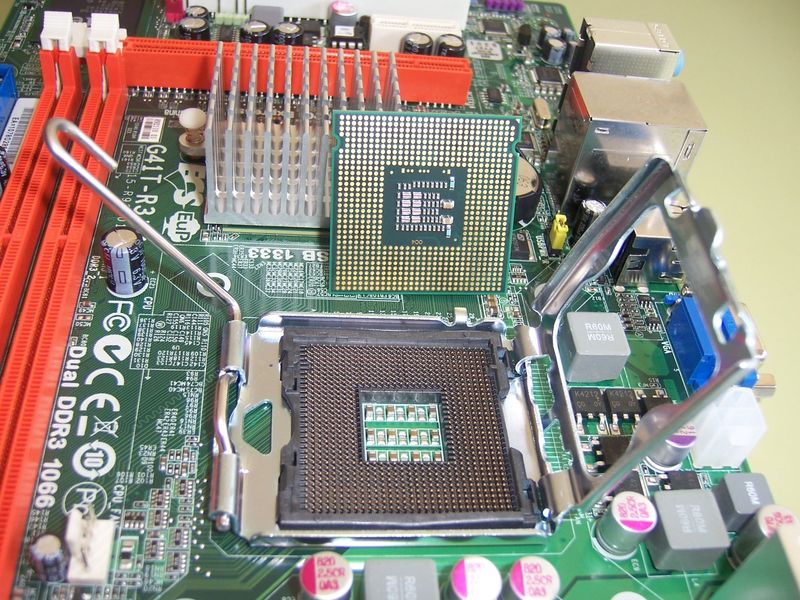
\includegraphics[scale=0.28]{mb-lga.JPG}
            \caption{Zócalo de tipo LGA}
        \end{figure}
    \end{itemize}

    Según el número de contactos y el tipo de distribución en el conector tendríamos una variedad bastante amplia de microprocesadores. La clasificación también depende del fabricante (AMD o Intel) y de sus gamas de modelos. A continuación se muestra una tabla con los principales zócalos empleados por ambos fabricantes:

        \begin{figure}[ht]

        \vspace{3ex}
        \centering

        \setlength{\tabcolsep}{10pt}
        \renewcommand{\arraystretch}{1.4}

        \begin{tabular}{| l | l |}
            \hline
            \centering\textbf{AMD}  & \textbf{Intel}  \\ \hline
            \centering Slot A: Duron, Athlon. &  Slot 1: Pentium II, Pentium III, Celeron. \\
            \centering Socket A: Duron, Athlon, Athlon XP &  Socket 370: Pentium III, Celeron \\
            \centering Socket 754: Athlon 64, Mobile Athlon 64 &  Socket 423: Pentium 4 \\
            \centering Socket 939: Athlon 64, Athlon FX &  Socket 478: Pentium 4, Celeron. \\
            \centering Socket 940: Opteron y Athlon 64 FX. &  Socket 775: Pentium 4, Celeron, Pentium D \\
            \centering Socket AM2: Athlon 64, Athlon FX, Athlon X2 &  Socket 603: Xeon \\
            \centering Socket F: Opteron. &  Socket 604: Xeon \\
            \centering Socket AM2+: Athlon 64, Athlon FX &  Socket 771: Xeon \\
            \centering Socket AM3: Phenom II, Athlon II &  LGA 1366: Intel Core i7, Xeon \\
            \centering Socket AM3+: FX Vishera, FX Zambezi &  LGA 1156: Intel Core i3, i5, i7. \\
            \centering Socket AM1: Athlon, Sempron. & LGA 2011: Core i7, Xeon E5 \\
            \centering Socket AM4: Ryzen 7, Ryzen 5, Ryzen 3 &  LGA 1150: Haswell, Broadwell \\
            \centering Socket TR4:  Ryzen Threadripper. &  LGA 1151: Skylake, Kaby Lake, Coffee Lake \\
            \centering  &  LGA 2066: Skylake-X, Kaby Lake-X \\
            \hline
        \end{tabular}
        \caption{Principales zócalos empleados por AMD y Intel}
    \end{figure}

    \item \textbf{Ranuras de Memoria}: Estos conectores son estrechos y alargados, de unos 13,1 centímetros. Tienen unas pestañas que sujetan las placas de memoria al ser insertadas con una ligera presión.

        \begin{figure}[ht]
        \centering
        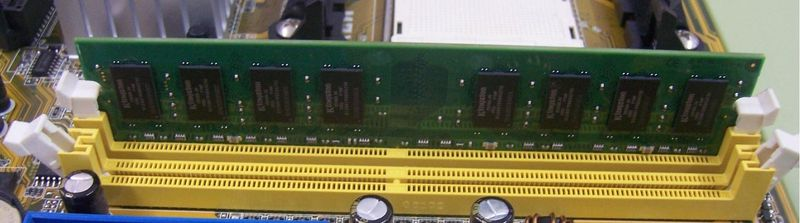
\includegraphics[scale=0.55]{conectores-RAM.jpg}
        \caption{Zócalo de memoria RAM}
    \end{figure}

    Suelen tener algún resalte que obliga a colocar las memorias en su posición correcta. El número de contactos varía según el tipo de memoria soportada por el chipset de la placa base, que por supuesto debe coincidir con el número de contactos de la placa de memoria.

    En la actualidad se usan los módulos de memoria DIMM con 4 variantes:
    \begin{itemize}
        \item DIMM de 168 pines para memorias SDRAM.
        \item DIMM de 184 pines para memorias DDR.
        \item DIMM de 240 pines para memorias DDR2 o DDR3.
        \item DIMM de 288 pines para memorias DDR4.
    \end{itemize}

    El número de zócalos de memoria suele variar en cada modelo de placa, pero suelen agruparse en bancos de 2 o 4 ranuras de memoria. Si una placa contiene dos tipos diferentes de ranuras será porque soporta la instalación de dos tipos diferentes de memoria, aunque no puedan usarse ambos tipos simultáneamente.

    \item \textbf{Ranuras de expansión}: Sirven para insertar en ellos tarjetas adaptadoras para conectar dispositivos periféricos, como la tarjeta de vídeo para conectar el monitor o la de sonido para conectar altavoces, etc...

    En las placas actuales podemos encontrar ranuras \textbf{PCI} y \textbf{PCI Express} de distintas velocidades. Cada una de ellas tiene sus propias características, variando en velocidad de transmisión, número de conexiones y tamaño.

        \begin{figure}[ht]
        \centering
        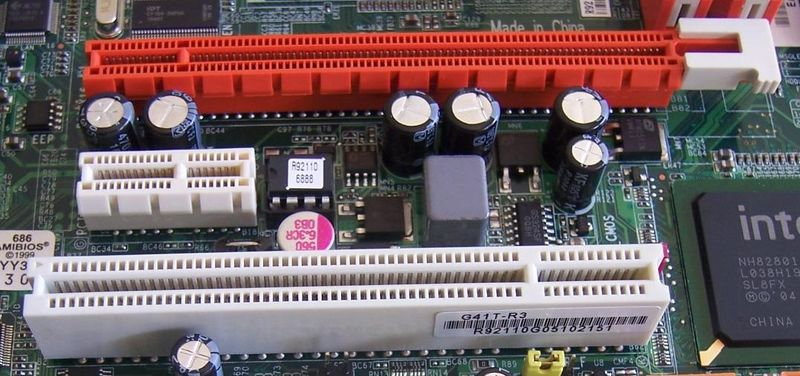
\includegraphics[scale=0.45]{conectores-PCI.jpg}
        \caption{Ranura de expansión PCI}
    \end{figure}

    Insertar una tarjeta en la ranura correspondiente es tan fácil como ejercer una ligera presión vertical para lograr que sus conectores se alojen en la ranura de expansión. A continuación, para evitar movimientos indeseados, las tarjetas van sujetas con un tornillo al chasis, mediante un tornillo situado en la placa metálica de la tarjeta, pudiendo así acceder a la nueva conexión desde el exterior del PC.

    \item \textbf{Conectores para Dispositivos Internos}: aquí vamos a incluir los conectores que se incluyen en las placas base para distintos usos:

    \begin{itemize}
        \item \textbf{Conectores para dispositivos de almacenamiento}: estos conectores se usan para ampliar el almacenamiento del ordenador y suelen ser de 3 tipos diferentes:

        \begin{itemize}
            \item \textbf{Conectores IDE}:
        \end{itemize}
    \end{itemize}
\end{itemize}




% Glossary

\glsaddall
\printglossaries

% Bibliography

\newpage
\addcontentsline{toc}{chapter}{Bibliografía}
\bibliography{citas}
\bibliographystyle{unsrt}

\end{document}